\documentclass{llncs}

\newcommand{\isDraft}{true}

\usepackage{amsmath}
\usepackage[usenames,dvipsnames]{color}
\usepackage{listings}
\usepackage[a4paper, top=2cm, bottom=3cm, left=2cm, right=2cm]{geometry}
\usepackage{graphicx}

\newcommand{\isDraft}{false}
\newcommand{\bfc}{{\sc Bfc}}
\newcommand{\mist}{{\sc Mist}}
\newcommand{\iic}{{\sc IIC}}
\newcommand{\pnerf}{{\sc Pnerf}}
\newcommand{\zthree}{{\sc Z3}}
\newcommand{\ttt}[1]{\texttt{#1}}

\usepackage{tikz}
\usetikzlibrary{arrows,shapes,shapes.multipart,shapes.geometric,
	snakes,automata,backgrounds,petri,calc,positioning}


\tikzstyle{place}=[circle,thick,draw=black!75,fill=white!20,
  	minimum size=6mm]
\tikzstyle{red place}=[place,draw=red!75,fill=red!20]
\tikzstyle{blue place}=[place,draw=blue!75,fill=blue!20]
\tikzstyle{transition}=[rectangle,thick,draw=black!75,
  	fill=black!20,minimum size=4mm]

\tikzstyle{state}=[draw, ellipse, aspect=2]
\tikzstyle{action}=[draw, rectangle, align=center]
\tikzstyle{decision}=[draw, diamond, aspect=2, align=center]
\tikzstyle{print}=[draw, trapezium, trapezium left angle=70, trapezium right angle=-70]
\tikzstyle{every edge}=[draw, ->, >=stealth, shorten >=2pt, shorten <=2pt]

\ifthenelse{\equal{\isDraft}{true}}{
  \usepackage[a4paper, top=2cm, bottom=3cm, left=2cm, right=2cm]{geometry}
  \pagestyle{plain}
}{}

\begin{document}

\nocite{DOsualdoSAS13}

\ifthenelse{\equal{\isDraft}{false}}{
  \title{An SMT-based Approach to Coverability Analysis}
  \author{
    Javier Esparza\inst{1}
    \and
    Rupak Majumdar\inst{2}
    \and
    Philipp Meyer\inst{1}
    \and
    Filip Niksic\inst{2}
    \and
    Rusl\'{a}n Ledesma-Garza\inst{1}
  }
  \institute{
    Technische Universit\"at M\"unchen
    \and
    MPI-SWS, Kaiserslautern and Saarbr\"ucken
  }
  
  \maketitle

  \begin{abstract}
    Model checkers based on Petri net coverability have been used
    successfully in recent years to verify safety properties of concurrent
    shared-memory or asynchronous message-passing software. The bottleneck
    in the verification process is the iterative computation of the
    (backward) reachable or (forward) coverable set, and most recent
    research has focused on non-trivial heuristics to speed it up.

    In this paper, we revisit a constraint approach to the problem based on
    classical Petri net analysis techniques: marking equation, place
    invariants, and traps. Given a marking M to be covered, the approach
    constructs constraints corresponding to increasingly precise
    overapproximations of the reachable markings covering M. If one of
    these constraints is unsatisfiable, then M is not coverable.

    Previous work on this approach suffered from the absence of efficient
    decision procedures for linear arithmetic, which nowadays exist as a
    part of SMT solvers. We show how to utilize an SMT solver to implement
    the constraint approach, and additionally, to generate a minimized
    inductive invariant from a safety proof.

    We empirically evaluate our procedure on a large set of existing Petri
    net benchmarks arising out of software verification. Surprisingly, even
    though our technique is incomplete, we show that it can quickly
    discharge all safe instances, usually competitive with, and occasionally
    much faster than, state-of-the-art techniques. Additionally, the
    inductive invariants computed are usually orders of magnitude smaller
    than those produced by existing solvers.
  \end{abstract}
}{
}


\section{Introduction}

This paper makes the following contributions.
\begin{itemize}
\item An application of \zthree\ to the constraint approach and its
  corresponding evaluation.
\item A method that given a network and a property constructs a
  minimal invariant.
\end{itemize}

\section{Illustration}

\section{Preliminaries}

A \emph{Petri net} is a tuple $(P, T, F, M_0)$, where $P$ is the set of
\emph{places}, $T$ is the set of \emph{transitions},
$F \subseteq P\times T \cup T\times P$ is the \emph{flow relation}
and $M_0$ is the initial marking.
We identify $F$ with its characteristic function
$P\times T \cup T\times P \to \{0, 1\}$.

For $x\in P\cup T$, the \emph{pre-set} is
$\pre{x}=\{y\in P\cup T\mid (y,x) \in F\}$
and the \emph{post-set} is $\post{x}=\{y\in P\cup T\mid (x,y) \in F\}$.
The pre- and post-set of a subset of $P \cup T$ are the union of
the pre and post-sets of its elements.

A \emph{marking} of a Petri net is a function $M\colon P \to \mathbb{N}$,
which describes the number of tokens $M(p)$ that the marking puts in
each place $p$.

Petri nets are represented graphically as follows: places and transitions
are represented as circles and boxes, respectively. An element $(x,y)$
of the flow relation is represented by an arc leading from $x$ to $y$.
A token on a place $p$ is represented by a black dot in the circle
corresponding to $p$.

A transition $t \in T$ is \emph{enabled at $M$} iff
$\forall p \in \pre{t} \colon M(p) \ge F(p, t)$.
If $t$ is enabled at $M$, then $t$ may \emph{fire} or \emph{occur},
yielding a new marking $M'$ (denoted as $M \xrightarrow{t} M'$),
where $M'(p) = M(p) + F(t,p) - F(p,t)$.

A sequence of transitions, $\sigma = t_1 t_2 \ldots t_r$ is an
$\emph{occurence sequence}$ of $N$ iff there exist markings
$M_1, \ldots, M_r$ such that $M_0 \xrightarrow{t_1} M_1
\xrightarrow{t_2} M_2 \ldots \xrightarrow{t_r} M_r$. The marking
$M_r$ is said to be \emph{reachable} from $M_0$ by the occurence
of $\sigma$ (denoted $M \xrightarrow{\sigma} M_r$).

A property $P$ is a safety property expressed over linear arithmetic
formulas. The property $P$ holds on a marking $M$ iff $M \models P$.
Examples of properties are $s_1 \le 2$, $s_1 + s_2 \ge 1$ and
$((s_1 \le 1) \land (s_2 \ge 1)) \lor (s_3 \le 1)$.

A Petri net $P$ satisfies a property $P$ (denoted by $N \models P$)
iff for all reachable markings $M_0 \xrightarrow{\sigma} M$
$M \models P$ holds.


\iffalse
\begin{verbatim}
 Examples:
  x + y < 0
  x + y < 0 \\and x + z > 0
  x + y < 0 \\or  x + z > 0

 ~P = (x + y <  0 \\and x + z >  0) \\or  x + z >  0
  P = (x + y >= 0 \\or  x + z <= 0) \\and x + z <= 0
\end{verbatim}
\fi


\newpage
\section{Method Safety}

The method Safety checks that a given Petri net \verb=N= never violates a property \verb=P=.
We present the method Safety by example on Lamport's 1-bit algorithm [Esparza1997].

\begin{verbatim}
* Method Safety:

  Subprocedure \mathcal{C} constructs state constraints C corresponding to N.
\end{verbatim}

\begin{center}
  \begin{tikzpicture}
    \node[state] (begin) {BEGIN};
    \node[action, below=of begin] (c) {$C:=\mathcal C(N)$};
    \node[decision, below=of c] (satc) {$\text{SAT}(C \cup \{\neg P\})$};
    \node[print, right=of satc] (yes) {N satisfies P};
    \node[print, below=of satc] (dontknow) {Don't know};
    \node[state, right=of yes] (end1) {END};
    \node[state, below=of dontknow] (end2) {END};
    
    \draw (begin) edge (c);
    \draw (c) edge (satc);
    \draw (satc) edge node[above]{NO} (yes);
    \draw (yes) edge (end1);
    \draw (satc) edge node[right]{YES} (dontknow);
    \draw (dontknow) edge (end2);
  \end{tikzpicture}
\end{center}

\begin{verbatim}
* Property of state constraints C: If C U {\neg P} is unsat then N |= P.

* Place equation:
  
  For a given place s the place equation is

  # of tokens in s = initial number of tokens of place s
                     + # times each input transition of s fires
                     - # times each output transition of s fires

* Non-negativity conditions:

  # of tokens in place s           >= 0
  # of times transition t is fired >= 0

* Subprocedure \mathcal{C}:

  Input:
    (S, T, E, M0) : Petri net
  Output:
    C : State constraints

  Pseudocode:

\end{verbatim}

\begin{align*}
  C(S, T, E, M_0) :=& \left( \bigwedge_{s \in S} \left(
    s = M_0(s) + \sum_{(t, s) \in E} t - \sum_{(s, t) \in E} t
  \right) \right) \land
    \left( \bigwedge_{s \in S} s \ge 0 \right) \land
    \left( \bigwedge_{t \in T} t \ge 0 \right)
\end{align*}

\newpage

\begin{verbatim}
* Example

  - Code:

  Process 1:                     |      Process 2:
                                 |
      bit1 := false              |      bit2 := false
      while true do              |      while true do
  p1:   bit1 := true             |  q1:   bit2 := true
  p2:   while bit2 do skip od    |  q2:   if bit1 then
  p3:   <critical section>       |  q3:     bit2 := true
        bit1 := false            |  q4:     while bit1 do skip od
      od                         |          goto q1
                                 |        fi
                                 |  q5:   <critical section>
                                 |        bit2 := false
                                 |      od

  - Property: Process 1 and Process 2 are never in their respective critical section at the same time.

  - Petri net:

\end{verbatim}

\begin{center}
  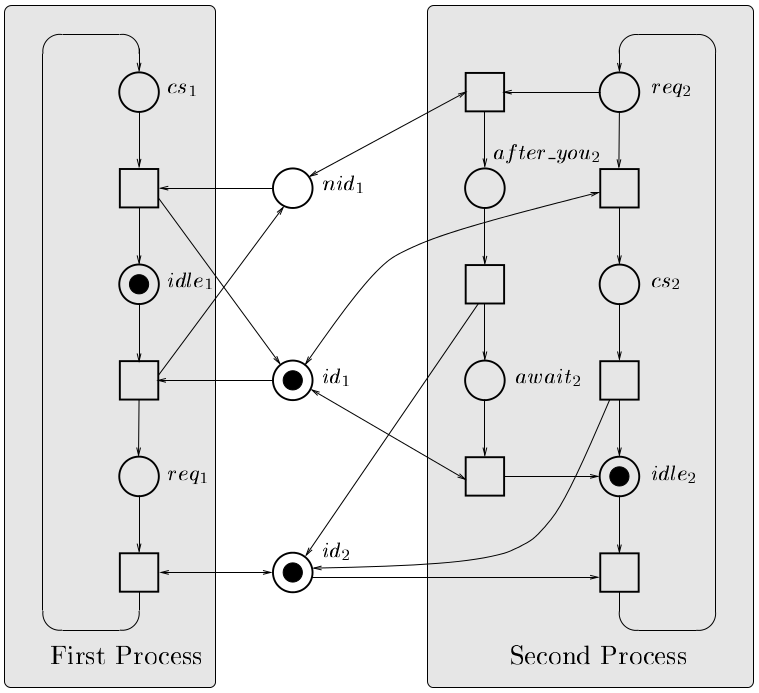
\includegraphics[width=10cm]{lamport}
\end{center}

\newpage

\begin{verbatim}
  - State constraints C:

    Place equations:
  
    a     = 1 + t1 - t2
    ^       ^   ^    ^
    |       |   |    |
    |       |   |    |
    |       |   |    |
    |       |   |   # of tokens taken from a
    |       |   |    
    |       |  # of tokens given to a
    |       |
    |      initial number of tokens in a
    |
    number of tokens in a

    b     = 0 - t1 + t2
    nbit2 = 0
    
    Non-negativity conditions:
  
    a     >= 0
    b     >= 0
    nbit2 >= 0

  - Negated Property \neg P:

    a + b >= 2
\end{verbatim}

\newpage

\section{Method Safety by Refinement}

The method Safety by Refinement applies trap conditions to check that a given Petri net \verb=N= never violates a property \verb=P=.

\begin{verbatim}
* Method Safety by Refinement:

  Subprocedure TrapConditions constructs trap conditions C_\theta corresponding to N and A.
  Subprocedure \Delta constructs refinement constraint \delta corresponding to A_\theta.
\end{verbatim}
\begin{center}
\begin{tikzpicture}
  \node[state] (begin) {BEGIN};
  \node[action, below=of begin] (c) {$C:=\mathcal C(N)$};
  \node[decision, below=of c] (satc) {$\text{SAT}(C \cup \{\neg P\})$};
  \node[action, below=of satc] (modelc) {$A:=\text{Model}(C \cup \{\neg P\})$\\
                               	$C_{\theta}:=\text{TrapConditions}(N, A)$};
  \node[decision, below=of modelc] (satctheta) {$\text{SAT}(C_\theta)$};
  \node[action, below=of satctheta] (modelctheta) {$A_\theta:=\text{Model}(C_\theta)$\\
                                    	$\delta:=\Delta(A_\theta)$\\
                                    	$C:=C \cup \{\delta\}$};
  \node[print, right=of satc] (yes) {N satisfies P};
  \node[print, right=of satctheta] (dontknow) {Don't know};
  \node[state, right=of yes] (end1) {END};
  \node[state, right=of dontknow] (end2) {END};

  \draw (begin) edge (c);
  \draw (c) edge coordinate[pos=.5] (edgein) (satc);
  \draw (satc) edge node[above]{NO} (yes);
  \draw (yes) edge (end1);
  \draw (satc) edge node[right]{YES} (modelc);
  \draw (modelc) edge (satctheta);
  \draw (satctheta) edge node[above]{NO} (dontknow);
  \draw (dontknow) edge (end2);
  \draw (satctheta) edge node[right]{YES} (modelctheta);
  \draw (modelctheta.south) -- ([yshift=-0.5cm] modelctheta.south)
  -| ([xshift=-2cm] modelctheta.west) |- (edgein);
\end{tikzpicture}
\end{center}

\begin{verbatim}
* Property of trap conditions C_\theta: If C_\theta is sat then there is a set S such that
  1. S is a trap in the net N
  2. S is marked in the initial marking M0
  3. S is unmarked in the assignment A

* Property of A_\theta: for each place s, A_\theta(s) iff s \in S

* Property of refinement constraint \delta: Constraint \delta refines the abstraction, i.e.
  1. A ^ \delta is unsat (\delta excludes A)
  2. N |= \delta is sat  (\delta is a property of N)
\end{verbatim}

\newpage

\begin{verbatim}
* Subprocedure TrapConditions:

  Input:
    (S, T, E, M0) : Petri net
    A             : Satisfying assignment for C \cup { ~P }
  Output:
    C_\theta      : Trap conditions

  Pseudocode:
  
\end{verbatim}
\begin{align*}
  C_\theta(S, T, E, M_0) :=& \left( \bigwedge_{s \in S} \left( s \Rightarrow
      \bigwedge_{(s, t) \in E} \bigvee_{(t, p) \in E} p
    \right) \right) \land
    \left( \bigvee_{s \in S: M_0(s) > 0} s \right) \land
    \left( \bigwedge_{s \in S: A(s) > 0} \neg s \right)
\end{align*}
\begin{verbatim}

* Subprocedure \Delta:

  Input:
    A_\theta      : Satisfying assignment for C_\theta
  Output:
    \delta        : Refinement constraint \delta

  Pseudocode:

\end{verbatim}
\begin{align*}
  & \delta(A_\theta) := \left( \sum_{A_\theta(s)} s \ge 0 \right)
\end{align*}

\newpage

\begin{verbatim}
* Example

  - State constraints C same as in the example for method Safety.
 
  - Property P:

    b = 0 
  
  - Negated Property \neg P:
    
    b >= 1

  - Assignment A:
    a     = 0
    b     = 1
    nbit2 = 0
    t1    = 0
    t2    = 1

  - Trap conditions C_\theta:

    - Trap implications:
               t2
             ----------
    a     => b \/ nbit2
    ^           ^      ^
    |           |      |
    |           |     nbit2 \in S
    |           |
    |          b \in S
    |
    a \in S
    
    nbit2 => b \/ nbit2
    b     => a

    - At least one of the initially marked places belongs to S:
    a

    - None of the marked places in A belongs to S:
    ~b
  
  - Assignment A_\theta:
    a     = true
    b     = false
    nbit2 = true

  - Refinement constraint \delta:
    a + b >= 1
    ^   ^
    |   |
    -----
      |
      S = {a, b}, therefore \delta excludes assignment A in the next iteration
\end{verbatim}

\newpage

\begin{verbatim}

* Trap implication:

  place s \in S =>    /\       \    /
                     /  \       \  /     place p \in S
                    /    \       \/
                   t \in s*   p \in t*   


  "if s is in trap S then for each output transition t at least one successor p is in trap S"


* Refinement constraint \delta:

  \Sigma s >= 1  
  A(s)

  "At least one place in S is always marked"
\end{verbatim}

\newpage

\section{Method Invariant}

The method Invariant constructs an invariant \verb=I= for given Petri net \verb=N= and \verb=P= when \verb=N= never violates \verb=P=.

\begin{verbatim}
* Code, property, and Petri net: same as in section Method Safety.
\end{verbatim}

\begin{verbatim}
* Method Invariant

  Subprocedure \mathcal{C'} constructs dual state constraints C' corresponding to N and P.
  Subprocedure Model returns assignment A such that A satisfies C'.
  Subprocedure Inv constructs invariant I corresponding to N and A'.
\end{verbatim}

\begin{center}
  \begin{tikzpicture}
    \node[state] (begin) {BEGIN};
    \node[action, below=of begin] (c) {$C':=\mathcal C'(N, \neg P)$};
    \node[decision, below=of c] (satc) {$\text{SAT}(C')$};
    \node[print, right=of satc] (noinv) {No Invariant};
    \node[action, below=of satc] (inv) {$A':=\text{Model}(C')$\\
      $I := \text{Inv}(N, A')$};
    \node[print, below=of inv] (printinv) {Invariant: $I$};
    \node[state, right=of noinv] (end1) {END};
    \node[state, below=of printinv] (end2) {END};
    
    \draw (begin) edge (c);
    \draw (c) edge (satc);
    \draw (satc) edge node[above]{NO} (noinv);
    \draw (satc) edge node[right]{YES} (inv);
    \draw (noinv) edge (end1);
    \draw (inv) edge (printinv);
    \draw (printinv) edge (end2);
  \end{tikzpicture}
\end{center}

\begin{verbatim}
* Property of dual state constraints C':  If C' is sat then N |= P.

* Property of invariant I:
  - I is reachable: For each reachable marking M, I(M) is valid
  - I is safe:      For markings that violate the property, I(M) is unsat
  - I is inductive: For each marking M, if I(M) is valid and M -> M1 then I(M1) is valid
\end{verbatim}

\newpage

\begin{verbatim}
* Subprocedure \mathcal{C'}:

  Input:
    N = (S, T, E, M0)  : Petri net
    \neg P = (p_1,1 + ... + p_1,m_1 >= b_1 /\ p_2,1 + ... + p_2,m_2 >= b_2 /\
              ... /\ p_n,1 + ... + p_n,m_n >= b_n ) : Negated property
  Output:
    C'            : Dual state constraints

Input:
 N      = (S, T, E, M0)
        = ( (a b nbit2 ) (t1 t2) (e1 ... en) (1 0 0) )
\neg P  = ( a + b >= 2 )

Pseudocode:
\end{verbatim}

\begin{align*}
  C'(N, \neg P) =& \left( \bigwedge_{t \in T} \left( 0 \ge
                      \sum_{(t, s) \in E} s
                    - \sum_{(s, t) \in E} s \right) \right) \land
     \left( \sum_{s \in S} M_0(s) \cdot s <
       \sum_{i=1}^n b_i \cdot target_i \right) \land \\
     & \left( \bigwedge_{s \in S} \left ( s \ge 
       \sum_{i : s \in \{ p_{i,1}, \ldots, p_{i,m_i} \} } target_i \right) \right) \land
     \left( \bigwedge_{i=1}^n \left( target_i \ge 0 \right) \right)
\end{align*}

\begin{verbatim}
* Subprocedure Inv:

  Input:
    N = (S, T, E, M0) : Petri net
    A'                : Satisfying assignment for C'

  Output:
    I                 : Invariant

  Pseudocode:
\end{verbatim}

\begin{align*}
  I(N, A') =& \left( \sum_{s \in S} A'(s) \cdot s \le
                     \sum_{s \in S} A'(s) \cdot M_0(s) \right)
\end{align*}

\newpage

\begin{verbatim}
* Derivation of invariant I for Petri net N that satisfies property P:

  M                                    : marking          ~ places
  C                                    : incidence matrix ~ rows correspond to places, columns correspond to transitions, relates places to transitions
  X                                    : firing vector    ~ transitions

  The following constraints C1 are unsat.
  M = M0 + C*X                         : place equations
  M >= 0                               : non-negativity conditions for places
  X >= 0                               : non-negativity conditions for transitions
  AM >= b                              : property P negated

  Substitute M to obtain constraints C2.
  A(M0 + CX) >= b                      : property P negated
  M0 + CX >= 0                         : non-negativity conditions for places
  X >= 0                               : non-negativity conditions for transitions

  Rewrite each system to obtain constraints C3.
  (-A*C)      (A*M0-b)                 : property P negated
  (  -C)*X <= (  M0  )                 : non-negativity conditions for places
  (  -I)      (   0  )                 : non-negativity conditions for transitions

  Apply Farkas' Lemma to obtain constraints C4.
  yT*(-A*C)                            : 
     (  -C) = 0                        : 
     (  -I)                            : 

  yT*(A*M0-b)                          : 
     (  M0  ) < 0                      : 
     (   0  )                          : 

  y >= 0                               : 

  The constraints C4 are sat iff the following constraints C5 are sat.
  y1 * A * C + y2 * C + y3 = 0         : 
  y1 * (A*M - b) + y2 * M0 < 0         : 
  y1 >= 0                              : 
  y2 >= 0                              : 
  y3 >= 0                              : 

  The constraints C5 are sat iff the following constraints C6 are sat.
  (y1 * A + y2) * C  <= 0              : 
  (y1 * A + y2) * M0 < y1 * b          : 
  y1 >= 0                              : 
  y2 >= 0                              : 

  The constraints C6 are sat iff the following constraints C' are sat.
  \lambda * C  <= 0                    : inductivity constraint
  \lambda * M0 < y1 * b                : safety constraint
  \lambda >= y1 * A                    : property constraint
  y1 >= 0                              : non-negativity constraint

  For \lambda satisfying C' the invariant is the following.
  I(M) = (\lambda * M <= \lambda * M0) : invariant
\end{verbatim}

\newpage

\begin{verbatim}
* Example:

  - Dual state constraints C':

    0        >=    a  - b
    0        >= (- a) + b

    a        <  2 * target_1

    a        >= target_1
    b        >= target_1
    nbit2    >= 0
    target_1 >= 0

  - Model A':

    a        = 1
    b        = 1
    nbit2    = 1
    target_1 = 1
    
  - Invariant:

    a + b + nbit2 <= 1

\end{verbatim}

\newpage

\section{Method Invariant with Minimization}

The method Invariant with Minimization constructs an invariant \verb=I=
that uses a minimal number of places for given Petri net \verb=N= and
\verb=P= when \verb=N= never violates \verb=P=. 

\begin{verbatim}
* Code, property, and Petri net: same as in section Method Safety.

* Method Invariant with Minimization

  Subprocedure \text{MinConstraints} constructs minimization constraints C_M corresponding to N and A'
\end{verbatim}

\begin{center}
  \begin{tikzpicture}
    \node[state] (begin) {BEGIN};
    \node[action, below=of begin] (c) {$C':=\mathcal C'(N, P)$};
    \node[decision, below=of c] (satc) {$\text{SAT}(C')$};
    \node[print, right=of satc] (noinv) {No Invariant};
    \node[action, below=of satc] (model1) {$A':=\text{Model}(C')$};
    \node[action, below=of model1] (cm) {$C_M:=\text{MinConstraints}(N, A')$};
    \node[decision, below=of cm] (satcm) {$\text{SAT}(C' \cup C_M)$};
    \node[action, right=of satcm] (model2) {$A':=\text{Model}(C' \cup C_M)$};
    \node[action, below=of satcm] (inv) {$I := \text{Inv}(N, A')$};
    \node[print, below=of inv] (printinv) {Invariant: $I$};
    \node[state, right=of noinv] (end1) {END};
    \node[state, below=of printinv] (end2) {END};
    
    \draw (begin) edge (c);
    \draw (c) edge (satc);
    \draw (satc) edge node[above]{NO} (noinv);
    \draw (noinv) edge (end1);
    \draw (satc) edge node[right]{YES} (model1);
    \draw (model1) edge coordinate[pos=.5] (edgein) (cm);
    \draw (cm) edge (satcm);
    \draw (satcm) edge node[above]{YES} (model2);
    \draw (model2) |- (edgein);
    \draw (satcm) edge node[right]{NO} (inv);
    \draw (inv) edge (printinv);
    \draw (printinv) edge (end2);
  \end{tikzpicture}
\end{center}

\begin{verbatim}
* Property of minimization constraints C_M generated from A': 
    If A'' satisfies C' u C_M, then Inv(N, A'') uses less places than Inv(N, A')
\end{verbatim}

\newpage

\begin{verbatim}
* Subprocedures \mathcal{C'} and Inv are the same as in Method Invariant

* Subprocedure \text{MinConstraints}:

  Input:
    N = (S, T, E, M0)  : Petri net
    A'                 : Satisfying assignment for C'
  Output:
    C_M                : Minimization Constraints

  Pseudocode:

\end{verbatim}

\begin{align*}
  C_M(N, A') =& \left( \bigwedge_{s \in S} \left(
      (s > 0 \Rightarrow b_s = 1) \land (s = 0 \Rightarrow b_s = 0)
    \right) \right) \land
    \left( \sum_{s \in S} b_s < \sum_{s \in S : A'(s) > 0} 1 \right)
\end{align*}

\newpage

\begin{verbatim}
* Example:

  - Dual state constraints C' and satisfying assignment A' for C' as in example for method Invariant

  - Minimization constraints C_M:

    a     > 0 => b_a     = 1
    |            -----------
    |               |
    |            place appears in invariant
    |
    place coefficient in the invariant

    a     = 0 => b_a     = 0
    |           ------------
    |               |
    |            place does not appear in invariant
    |
    place coefficient in the invariant

    b     > 0 => b_b     = 1
    b     = 0 => b_b     = 0
    nbit2 > 0 => b_nbit2 = 1
    nbit2 = 0 => b_nbit2 = 0

    b_a + b_b + b_nbit2 < 3
    -------------------   |
                |         |
                |    number of places appearing in current invariant for A'
                |    = #{s | A'(s) > 0} = #{a, b, nbit2}
                |
  number of places appearing in new invariant
  
  - Model A' for C' \cup C_M:

    a        = 1
    b        = 1
    nbit2    = 0
    target_1 = 1
    
  - Minimized Invariant:

    a + b <= 1
\end{verbatim}
    
\newpage

\section{Method Invariant by Refinement}

\begin{verbatim}
* Code, property, and Petri net: same as in section Method Safety by Refinement.

* Method Invariant by Refinement
\end{verbatim}

\begin{tikzpicture}
  \node[state] (begin) {BEGIN};
  \node[action, below=of begin] (c) {$C:=\mathcal C(N)$\\
                                        $D:=\{\}$};
  \node[decision, below=of c] (satc) {$\text{SAT}(C \cup \{\neg P\})$};
  \node[action, below=of satc] (modelc) {$A:=\text{Model}(C \cup \{\neg P\})$\\
                                        $C_{\theta}:=\text{TrapConditions}(N, A)$};
  \node[decision, below=of modelc] (satctheta) {$\text{SAT}(C_\theta)$};
  \node[action, below=of satctheta] (modelctheta) {$A_\theta:=\text{Model}(C_\theta)$\\
                                                $\delta:=\Delta(A_\theta)$\\
                                                $C:=C \cup \{\delta\}$\\
                                                $D:=D \cup \{\delta\}$};
  \node[print, right=of satctheta] (noinv2) {No Invariant};
  \node[state, below=of noinv2] (end3) {END};
   
  \node[action, right=of satc] (cprime) {$C':=\mathcal C'(N, \neg P \land D)$};
  \node[decision, right=of cprime] (satcprime) {$\text{SAT}(C')$};
  \node[action, below=of satcprime] (inv) {$A':=\text{Model}(C')$\\
                                        $I:=D \land \text{Inv}(N, A')$};
  \node[print, below=of inv] (printinv) {Invariant: $I$};
  \node[print, right=of satcprime] (noinv) {No Invariant};
  \node[state, below=of noinv] (end1) {END};
  \node[state, below=of printinv] (end2) {END};
 
  \draw (cprime) edge (satcprime);
  \draw (satcprime) edge node[above]{NO} (noinv);
  \draw (satcprime) edge node[right]{YES} (inv);
  \draw (inv) edge (printinv);
  \draw (noinv) edge (end1);
  \draw (printinv) edge (end2);
 
  \draw (begin) edge (c);
  \draw (c) edge coordinate[pos=.5] (edgein) (satc);
  \draw (satc) edge node[above]{NO} (cprime);
  \draw (satc) edge node[right]{YES} (modelc);
  \draw (modelc) edge (satctheta);
  \draw (satctheta) edge node[above]{NO} (noinv2);
  \draw (noinv2) edge (end3);
  \draw (satctheta) edge node[right]{YES} (modelctheta);
  \draw (modelctheta.south) -- ([yshift=-0.5cm] modelctheta.south)
  -| ([xshift=-2cm] modelctheta.west) |- (edgein);
\end{tikzpicture}

\begin{verbatim}
* Subprocedures TrapConditions and \Delta are the same as
  in Method Safety by Refinement

* Subprocedures \mathcal{C'} and Inv are the same as
  in Method Invariant
\end{verbatim}

\newpage

\begin{verbatim}
* Example:

  - Trap constraints as in example from section Method Safety by Refinement.
  
  - Dual state constraints C':

    0        >=    a  - b
    0        >= (- a) + b

    a        <  target_1 + trap_1

    a        >= trap_1
    b        >= target_1
    nbit2    >= trap_1
    target_1 >= 0
    trap_1   >= 0

  - Model A':

    a        = 1
    b        = 1
    nbit2    = 1
    target_1 = 1
    trap_1   = 1
    
  - Invariant:

    a     + nbit2 >= 1
    a + b + nbit2 <= 1
\end{verbatim}

\section{Experimental Evaluation}
\label{sec_experiments}

We have implemented our algorithms in a tool called
\emph{Pe\-tri\-ni\-zer}. 
Petrinizer is implemented as a combination of Bash and Prolog scripts,
and uses Z3 \cite{MouraB08} as a backend SMT solver.
It takes as input coverability problem instances encoded in the MIST
input format\footnote{\url{https://github.com/pierreganty/mist}}, and it
runs one of the selected methods. 
We implemented all possible combinations of
methods: with and without trap refinement, with real and integer arithmetic,
with and without invariant construction, with and without invariant
minimization.

The evaluation of Petrinizer had two main goals. First, as the underlying
methods are incomplete, we wanted to measure their success rate on standard
benchmark sets. 
As a subgoal, we wanted to investigate
the usefulness and necessity of traps, the benefit of using integer arithmetic
over real arithmetic, and the sizes of the constructed invariants.
The second goal was to measure Petrinizer's performance and to compare it
with state-of-the-art tools: IIC \cite{KloosMNP13}, BFC\footnote{The most recent version of BFC at the time of
writing the paper was 2.0. However, we noticed it sometimes reports
inconsistent results, so we used version 1.0 instead. The tool can be
obtained at \url{http://www.cprover.org/bfc/}.} \cite{KaiserKWCONCUR12}, and
MIST\footnote{MIST consists of several methods, most of them based on
  EEC \cite{GeeraertsRB06}. We used the abstraction
  refinement method that tries to minimize the number of places in the net \cite{GantyFI08}.}.

\paragraph{Benchmarks.} For the inputs used in the experiments, we collected a
large number of coverability problem instances originating from various sources. The
collection contains 178 examples, out of which 115 are safe, and is
organized into five example suites. The first suite is a collection of
Petri net examples from the MIST toolkit. This suite contains a
mixture of 29 examples, both safe and unsafe. It contains both real-world and
artificially created examples. The second suite consists of 46 Petri nets
that were used in the evaluation of BFC \cite{KaiserKWCONCUR12}. They
originate from the analysis of concurrent C programs, and they are mostly
unsafe. The third and the forth suite come from the
provenance analysis of messages in a medical and a bug-tracking system
\cite{MajumdarSAS13}. The medical suite contains 12 safe
examples, and the bug-tracking suite contains 41 examples, all
safe except for one. The final, fifth suite contains 50 examples that
come from the analysis of Erlang programs \cite{DOsualdoSAS13}. We generated
them ourselves using an Erlang verification tool Soter \cite{DOsualdoSAS13},
from the example programs found on Soter's
website\footnote{http://mjolnir.cs.ox.ac.uk/soter/}. Out of 50 examples in this
suite, 38 are safe. This suite also contains the largest example in the
collection, with 66,950 places and 213,635 transitions.
For our evaluation, only the 115 safe instances are interesting.

\begin{table}[t]
  \centering
  \caption{Safe examples that were successfully proved safe.}
  \label{table:rate-of-success}
  \scriptsize
  \begin{tabular}{|l|r|r|r|r|r|r|r|}
    \hline
    \multicolumn{1}{|c|}{Suite} & \multicolumn{1}{|c|}{Safety}
    & \multicolumn{1}{|c|}{Ref./reals} & \multicolumn{1}{|c|}{Ref./ints}
    & \multicolumn{1}{|c|}{IIC} & \multicolumn{1}{|c|}{BFC}
    & \multicolumn{1}{|c|}{MIST} & \multicolumn{1}{|c|}{Total} \\
    \hline
    MIST        & 14 & 20 & 20 & {\bf 23} & 21 & 19 & 23 \\
    BFC          & {\bf 2} & {\bf 2} & {\bf 2} & {\bf 2} & {\bf 2} & {\bf 2} & 2 \\
    Medical      & 4 & 4 & 4 & 9 & {\bf 12} & 10 & 12 \\
    Bug-tracking & {\bf 32} & {\bf 32} & {\bf 32} & 0 & - & 0 & 40 \\
    Erlang       & 32 & 36 & {\bf 38} & 17 & 26 & 2 & 38 \\
    \hline
    Total        & 84 & 94 & {\bf 96} & 51 & 61 & 33 & 115 \\
    \hline
  \end{tabular}
\end{table}

\paragraph{Rate of success on safe examples.} As shown in Table
\ref{table:rate-of-success}, even with the weakest of the methods---safety based
on marking equation over reals---Petrinizer is able to prove safety for 84 out
of 115 examples. Switching to integer arithmetic does not help: The number of
examples proved safe remains 84. Using refinement via traps, Petrinizer proves
safety for 94 examples. Switching to integer arithmetic in this case helps:
Another two examples are proved safe, totaling with 96 out of 115 examples. In
contrast to these numbers, the most successful existing tool turned out to be BFC, proving safety for
only 61 examples\footnote{This number comes with a caveat: We were not able to
run BFC on the bug-tracking suite, as the examples were too big for the tool that translates
MIST format into BFC format. For the BFC and Erlang suites, which contain
some similarly large or even larger examples, we initially had the inputs in BFC
format, and translated them into MIST format, thus avoiding the issue. Translation
utilities are provided by the authors of BFC.}. The small numbers are due to
time and memory limits. Even though the methods these tools implement
are complete, the tools themselves are limited by the time and space they can
use.

Looking at the results accross different suites, we see that Petrinizer
performed poorest on the medical suite, proving safety for only 4 out of 12
examples. On the other hand, on the bug-tracking suite, which was completely
intractable for other tools, it proved safety for 32 out of 40 examples.
Furthermore, using traps and integer arithmetic, Petrinizer successfuly proved
safety for all safe Erlang examples. We find this result particularly
surprising, as the original verification problems for these examples seem non-trivial.

\begin{figure}[t]
  \centering
  \begin{tikzpicture}[gnuplot]
%% generated with GNUPLOT 4.6p3 (Lua 5.1; terminal rev. 99, script rev. 100)
%% Sun Feb  9 20:56:35 2014
\path (0.000,0.000) rectangle (8.000,3.500);
\gpcolor{color=gp lt color border}
\gpsetlinetype{gp lt border}
\gpsetlinewidth{1.00}
\draw[gp path] (1.380,0.985)--(1.560,0.985);
\node[gp node right] at (1.196,0.985) {{\tiny $10^{0}$}};
\draw[gp path] (1.380,1.700)--(1.560,1.700);
\node[gp node right] at (1.196,1.700) {{\tiny $10^{1}$}};
\draw[gp path] (1.380,2.416)--(1.560,2.416);
\node[gp node right] at (1.196,2.416) {{\tiny $10^{2}$}};
\draw[gp path] (1.380,3.131)--(1.560,3.131);
\node[gp node right] at (1.196,3.131) {{\tiny $10^{3}$}};
\draw[gp path] (1.380,0.985)--(1.380,1.165);
\node[gp node center] at (1.380,0.677) {{\tiny $10^{0}$}};
\draw[gp path] (1.793,0.985)--(1.793,1.165);
\node[gp node center] at (1.793,0.677) {{\tiny $10^{1}$}};
\draw[gp path] (2.207,0.985)--(2.207,1.165);
\node[gp node center] at (2.207,0.677) {{\tiny $10^{2}$}};
\draw[gp path] (2.620,0.985)--(2.620,1.165);
\node[gp node center] at (2.620,0.677) {{\tiny $10^{3}$}};
\draw[gp path] (3.034,0.985)--(3.034,1.165);
\node[gp node center] at (3.034,0.677) {{\tiny $10^{4}$}};
\draw[gp path] (3.447,0.985)--(3.447,1.165);
\node[gp node center] at (3.447,0.677) {{\tiny $10^{5}$}};
\draw[gp path] (1.380,3.131)--(1.380,0.985)--(3.447,0.985)--(3.447,3.131)--cycle;
\node[gp node center,rotate=-270] at (0.306,2.058) {Size of invariant};
\node[gp node center] at (2.413,0.215) {Number of places};
\gpcolor{color=gp lt color 2}
\gpsetpointsize{2.00}
\gppoint{gp mark 7}{(1.826,1.700)}
\gppoint{gp mark 7}{(1.669,1.700)}
\gppoint{gp mark 7}{(2.283,2.544)}
\gppoint{gp mark 7}{(1.978,1.997)}
\gppoint{gp mark 7}{(2.373,2.702)}
\gppoint{gp mark 7}{(2.373,2.702)}
\gppoint{gp mark 7}{(2.093,2.206)}
\gppoint{gp mark 7}{(1.854,1.416)}
\gppoint{gp mark 7}{(1.935,1.200)}
\gppoint{gp mark 7}{(1.935,1.416)}
\gppoint{gp mark 7}{(2.002,1.416)}
\gppoint{gp mark 7}{(2.089,1.416)}
\gppoint{gp mark 7}{(1.899,1.700)}
\gppoint{gp mark 7}{(1.702,1.700)}
\gppoint{gp mark 7}{(1.878,1.416)}
\gppoint{gp mark 7}{(1.811,1.757)}
\gppoint{gp mark 7}{(1.878,1.805)}
\gppoint{gp mark 7}{(1.774,1.668)}
\gppoint{gp mark 7}{(1.854,1.883)}
\gppoint{gp mark 7}{(1.841,1.416)}
\gppoint{gp mark 7}{(2.411,1.200)}
\gppoint{gp mark 7}{(2.411,1.200)}
\gppoint{gp mark 7}{(2.411,1.200)}
\gppoint{gp mark 7}{(2.411,1.200)}
\gppoint{gp mark 7}{(2.570,1.846)}
\gppoint{gp mark 7}{(2.570,1.846)}
\gppoint{gp mark 7}{(2.570,1.846)}
\gppoint{gp mark 7}{(2.570,1.846)}
\gppoint{gp mark 7}{(2.570,1.200)}
\gppoint{gp mark 7}{(2.570,1.200)}
\gppoint{gp mark 7}{(2.570,1.200)}
\gppoint{gp mark 7}{(2.570,1.200)}
\gppoint{gp mark 7}{(2.570,1.200)}
\gppoint{gp mark 7}{(2.570,1.200)}
\gppoint{gp mark 7}{(2.570,1.200)}
\gppoint{gp mark 7}{(2.570,1.200)}
\gppoint{gp mark 7}{(2.570,1.200)}
\gppoint{gp mark 7}{(2.570,1.200)}
\gppoint{gp mark 7}{(2.570,1.200)}
\gppoint{gp mark 7}{(2.570,1.200)}
\gppoint{gp mark 7}{(2.570,1.200)}
\gppoint{gp mark 7}{(2.570,1.200)}
\gppoint{gp mark 7}{(2.570,1.200)}
\gppoint{gp mark 7}{(2.570,1.200)}
\gppoint{gp mark 7}{(2.570,1.200)}
\gppoint{gp mark 7}{(2.570,1.200)}
\gppoint{gp mark 7}{(2.570,1.200)}
\gppoint{gp mark 7}{(2.570,1.200)}
\gppoint{gp mark 7}{(2.570,1.200)}
\gppoint{gp mark 7}{(2.570,1.200)}
\gppoint{gp mark 7}{(2.570,1.200)}
\gppoint{gp mark 7}{(2.570,1.200)}
\gppoint{gp mark 7}{(2.570,1.200)}
\gppoint{gp mark 7}{(2.570,1.200)}
\gppoint{gp mark 7}{(2.570,1.200)}
\gppoint{gp mark 7}{(2.570,1.200)}
\gppoint{gp mark 7}{(2.514,2.071)}
\gppoint{gp mark 7}{(2.686,2.556)}
\gppoint{gp mark 7}{(2.900,3.067)}
\gppoint{gp mark 7}{(2.476,2.107)}
\gppoint{gp mark 7}{(2.476,2.107)}
\gppoint{gp mark 7}{(2.576,0.985)}
\gppoint{gp mark 7}{(2.870,0.985)}
\gppoint{gp mark 7}{(2.160,1.865)}
\gppoint{gp mark 7}{(2.184,1.945)}
\gppoint{gp mark 7}{(2.184,1.945)}
\gppoint{gp mark 7}{(2.341,1.700)}
\gppoint{gp mark 7}{(2.751,2.764)}
\gppoint{gp mark 7}{(2.678,2.648)}
\gppoint{gp mark 7}{(2.437,1.985)}
\gppoint{gp mark 7}{(2.526,2.009)}
\gppoint{gp mark 7}{(2.586,2.042)}
\gppoint{gp mark 7}{(2.564,1.985)}
\gppoint{gp mark 7}{(2.889,2.009)}
\gppoint{gp mark 7}{(3.037,2.031)}
\gppoint{gp mark 7}{(2.449,1.959)}
\gppoint{gp mark 7}{(2.961,2.365)}
\gppoint{gp mark 7}{(3.375,2.795)}
\gppoint{gp mark 7}{(2.388,2.668)}
\gppoint{gp mark 7}{(2.388,2.668)}
\gppoint{gp mark 7}{(2.388,2.662)}
\gppoint{gp mark 7}{(2.388,2.662)}
\gppoint{gp mark 7}{(2.388,1.846)}
\gppoint{gp mark 7}{(2.388,1.846)}
\gppoint{gp mark 7}{(2.380,2.098)}
\gppoint{gp mark 7}{(2.667,2.507)}
\gppoint{gp mark 7}{(2.777,2.666)}
\gppoint{gp mark 7}{(2.380,2.098)}
\gppoint{gp mark 7}{(2.380,2.098)}
\gppoint{gp mark 7}{(2.510,1.846)}
\gppoint{gp mark 7}{(2.510,1.826)}
\gppoint{gp mark 7}{(3.168,2.945)}
\gppoint{gp mark 7}{(2.343,1.985)}
\gppoint{gp mark 7}{(2.224,1.590)}
\gpcolor{color=gp lt color border}
\draw[gp path] (1.380,3.131)--(1.380,0.985)--(3.447,0.985)--(3.447,3.131)--cycle;
%% coordinates of the plot area
\gpdefrectangularnode{gp plot 1}{\pgfpoint{1.380cm}{0.985cm}}{\pgfpoint{3.447cm}{3.131cm}}
\draw[gp path] (5.380,0.985)--(5.560,0.985);
\node[gp node right] at (5.196,0.985) {{\tiny $10^{0}$}};
\draw[gp path] (5.380,1.414)--(5.560,1.414);
\node[gp node right] at (5.196,1.414) {{\tiny $10^{1}$}};
\draw[gp path] (5.380,1.843)--(5.560,1.843);
\node[gp node right] at (5.196,1.843) {{\tiny $10^{2}$}};
\draw[gp path] (5.380,2.273)--(5.560,2.273);
\node[gp node right] at (5.196,2.273) {{\tiny $10^{3}$}};
\draw[gp path] (5.380,2.702)--(5.560,2.702);
\node[gp node right] at (5.196,2.702) {{\tiny $10^{4}$}};
\draw[gp path] (5.380,3.131)--(5.560,3.131);
\node[gp node right] at (5.196,3.131) {{\tiny $10^{5}$}};
\draw[gp path] (5.380,0.985)--(5.380,1.165);
\node[gp node center] at (5.380,0.677) {{\tiny $10^{0}$}};
\draw[gp path] (6.069,0.985)--(6.069,1.165);
\node[gp node center] at (6.069,0.677) {{\tiny $10^{1}$}};
\draw[gp path] (6.758,0.985)--(6.758,1.165);
\node[gp node center] at (6.758,0.677) {{\tiny $10^{2}$}};
\draw[gp path] (7.447,0.985)--(7.447,1.165);
\node[gp node center] at (7.447,0.677) {{\tiny $10^{3}$}};
\draw[gp path] (5.380,3.131)--(5.380,0.985)--(7.447,0.985)--(7.447,3.131)--cycle;
\node[gp node center,rotate=-270] at (4.306,2.058) {IIC};
\node[gp node center] at (6.413,0.215) {Petrinizer};
\gpcolor{color=gp lt color 0}
\gpsetlinetype{gp lt plot 0}
\draw[gp path] (5.380,0.985)--(5.397,0.995)--(5.413,1.006)--(5.430,1.016)--(5.447,1.027)%
  --(5.464,1.037)--(5.480,1.047)--(5.497,1.058)--(5.514,1.068)--(5.530,1.079)--(5.547,1.089)%
  --(5.564,1.099)--(5.580,1.110)--(5.597,1.120)--(5.614,1.131)--(5.631,1.141)--(5.647,1.151)%
  --(5.664,1.162)--(5.681,1.172)--(5.697,1.183)--(5.714,1.193)--(5.731,1.203)--(5.747,1.214)%
  --(5.764,1.224)--(5.781,1.235)--(5.798,1.245)--(5.814,1.255)--(5.831,1.266)--(5.848,1.276)%
  --(5.864,1.287)--(5.881,1.297)--(5.898,1.308)--(5.914,1.318)--(5.931,1.328)--(5.948,1.339)%
  --(5.965,1.349)--(5.981,1.360)--(5.998,1.370)--(6.015,1.380)--(6.031,1.391)--(6.048,1.401)%
  --(6.065,1.412)--(6.081,1.422)--(6.098,1.432)--(6.115,1.443)--(6.132,1.453)--(6.148,1.464)%
  --(6.165,1.474)--(6.182,1.484)--(6.198,1.495)--(6.215,1.505)--(6.232,1.516)--(6.248,1.526)%
  --(6.265,1.536)--(6.282,1.547)--(6.299,1.557)--(6.315,1.568)--(6.332,1.578)--(6.349,1.588)%
  --(6.365,1.599)--(6.382,1.609)--(6.399,1.620)--(6.415,1.630)--(6.432,1.640)--(6.449,1.651)%
  --(6.466,1.661)--(6.482,1.672)--(6.499,1.682)--(6.516,1.692)--(6.532,1.703)--(6.549,1.713)%
  --(6.566,1.724)--(6.582,1.734)--(6.599,1.744)--(6.616,1.755)--(6.633,1.765)--(6.649,1.776)%
  --(6.666,1.786)--(6.683,1.796)--(6.699,1.807)--(6.716,1.817)--(6.733,1.828)--(6.749,1.838)%
  --(6.766,1.848)--(6.783,1.859)--(6.800,1.869)--(6.816,1.880)--(6.833,1.890)--(6.850,1.901)%
  --(6.866,1.911)--(6.883,1.921)--(6.900,1.932)--(6.916,1.942)--(6.933,1.953)--(6.950,1.963)%
  --(6.967,1.973)--(6.983,1.984)--(7.000,1.994)--(7.017,2.005)--(7.033,2.015);
\gpcolor{color=gp lt color 2}
\gppoint{gp mark 7}{(6.069,1.414)}
\gppoint{gp mark 7}{(6.069,1.414)}
\gppoint{gp mark 7}{(6.881,2.855)}
\gppoint{gp mark 7}{(6.355,2.200)}
\gppoint{gp mark 7}{(7.033,3.045)}
\gppoint{gp mark 7}{(7.033,3.045)}
\gppoint{gp mark 7}{(6.557,2.451)}
\gppoint{gp mark 7}{(5.795,1.722)}
\gppoint{gp mark 7}{(5.587,1.243)}
\gppoint{gp mark 7}{(5.795,1.448)}
\gppoint{gp mark 7}{(5.795,1.502)}
\gppoint{gp mark 7}{(5.795,1.502)}
\gppoint{gp mark 7}{(6.069,2.420)}
\gppoint{gp mark 7}{(6.069,1.585)}
\gppoint{gp mark 7}{(5.795,2.007)}
\gppoint{gp mark 7}{(6.124,1.797)}
\gppoint{gp mark 7}{(6.170,1.854)}
\gppoint{gp mark 7}{(6.037,1.804)}
\gppoint{gp mark 7}{(6.245,1.964)}
\gppoint{gp mark 7}{(5.795,1.954)}
\gppoint{gp mark 7}{(5.587,1.114)}
\gppoint{gp mark 7}{(5.587,1.114)}
\gppoint{gp mark 7}{(5.587,1.114)}
\gppoint{gp mark 7}{(5.587,1.114)}
\gppoint{gp mark 7}{(5.380,0.985)}
\gppoint{gp mark 7}{(5.380,0.985)}
\gppoint{gp mark 7}{(6.228,1.974)}
\gppoint{gp mark 7}{(6.305,2.031)}
\gppoint{gp mark 7}{(6.305,2.031)}
\gppoint{gp mark 7}{(6.069,2.049)}
\gppoint{gp mark 7}{(6.318,2.244)}
\gppoint{gp mark 7}{(6.995,2.190)}
\gppoint{gp mark 7}{(6.995,2.190)}
\gppoint{gp mark 7}{(6.210,2.392)}
\gppoint{gp mark 7}{(6.210,2.392)}
\gppoint{gp mark 7}{(6.452,2.435)}
\gppoint{gp mark 7}{(6.452,2.467)}
\gppoint{gp mark 7}{(6.210,2.086)}
\gppoint{gp mark 7}{(6.190,2.016)}
\gppoint{gp mark 7}{(6.343,1.585)}
\gppoint{gp mark 7}{(5.962,1.348)}
\gpcolor{color=gp lt color border}
\gpsetlinetype{gp lt border}
\draw[gp path] (5.380,3.131)--(5.380,0.985)--(7.447,0.985)--(7.447,3.131)--cycle;
%% coordinates of the plot area
\gpdefrectangularnode{gp plot 2}{\pgfpoint{5.380cm}{0.985cm}}{\pgfpoint{7.447cm}{3.131cm}}
\end{tikzpicture}
%% gnuplot variables

  \caption{Graph on the left shows a relation of sizes of constructed
  invariants to the number of places in the corresponding Petri nets. Graph
  on the right shows comparison in size of invariants produced by Petrinizer and
  IIC. Axes represent size on a logarithmic scale. Each dot represents one example.}
  \label{fig:invariant-size}
\end{figure}

\paragraph{Invariant sizes.} As the invariant construction is a new addition to
the existing methods, we wanted to inspect sizes of the constructed invariants.
We took the number of atomic terms appearing in an invariant's linear expressions
as a measure of its size. When we relate sizes of invariants to number of places
in the corresponding Petri net (left graph in Fig.~\ref{fig:invariant-size}), we
see that invariants are most of the times very succinct. As an example, the
largest invariant had 814 atomic terms, and the corresponding Petri net, coming
from the Erlang suite, had 4,763 places. For the largest Petri net in the
collection, the one with 66,950 places, the constructed invariant had 339 atomic
terms.

We also compared sizes of constructed invariants with
sizes of invariants produced by IIC \cite{KloosMNP13}. IIC's invariants
are expressed as CNF formulas over atoms of the form $x<a$,
for a variable $x$ and a constant $a$. As a measure of size for these formulas,
we took the number of atoms they contain. As the right graph in
Fig.~\ref{fig:invariant-size} shows, when compared to IIC's invariants, Petrinizer's invariants
are never larger, and are often orders of magnitude smaller.

\paragraph{Performance.} To ensure accuracy and fairness, all experiments were
performed on identical machines, equipped with Intel Xeon 2.66 GHz CPUs and 48 GB of memory, running Linux 3.2.48.1
in 64-bit mode. Execution time was limited to 100,000 seconds (27
hours, 46 minutes and 40 seconds), and memory to 2 GB.

Due to dissimilarities between the compared tools, selecting a fair
measure of time turned out to be tricky. On the one hand, as
Petrinizer communicates with Z3 via temporary files, it spends a
considerable amount of time doing I/O operations.  On the other hand,
as BFC performs both a forward and a backward search, it naturally
splits the work into two threads, and runs them in parallel on two CPU
cores. In both cases, the actual elapsed time does not quite
correspond to the amount of computational effort we wanted to measure.
Therefore, for the measure of time we selected the \emph{user time},
as reported by the \emph{time} utility on Linux. User time measures
the total CPU time spent executing the process and its children. In
the case of Petrinizer, it excludes the I/O overhead, and in the case
of BFC, it includes total CPU time spent on both CPU cores.

\begin{figure}[t]
  \centering
  \begin{tikzpicture}[gnuplot]
%% generated with GNUPLOT 4.6p3 (Lua 5.1; terminal rev. 99, script rev. 100)
%% Sun Feb  9 21:00:45 2014
\path (0.000,0.000) rectangle (12.500,3.500);
\gpcolor{color=gp lt color border}
\gpsetlinetype{gp lt border}
\gpsetlinewidth{1.00}
\draw[gp path] (1.564,0.985)--(1.744,0.985);
\node[gp node right] at (1.380,0.985) {{\tiny $10^{-1}$}};
\draw[gp path] (1.564,1.700)--(1.744,1.700);
\node[gp node right] at (1.380,1.700) {{\tiny $10^{0}$}};
\draw[gp path] (1.564,2.416)--(1.744,2.416);
\node[gp node right] at (1.380,2.416) {{\tiny $10^{1}$}};
\draw[gp path] (1.564,3.131)--(1.744,3.131);
\node[gp node right] at (1.380,3.131) {{\tiny $10^{2}$}};
\draw[gp path] (1.564,0.985)--(1.564,1.165);
\node[gp node center] at (1.564,0.677) {{\tiny $10^{-1}$}};
\draw[gp path] (2.247,0.985)--(2.247,1.165);
\node[gp node center] at (2.247,0.677) {{\tiny $10^{0}$}};
\draw[gp path] (2.931,0.985)--(2.931,1.165);
\node[gp node center] at (2.931,0.677) {{\tiny $10^{1}$}};
\draw[gp path] (3.614,0.985)--(3.614,1.165);
\node[gp node center] at (3.614,0.677) {{\tiny $10^{2}$}};
\draw[gp path] (1.564,3.131)--(1.564,0.985)--(3.614,0.985)--(3.614,3.131)--cycle;
\node[gp node center,rotate=-270] at (0.306,2.058) {Ref. over integers};
\node[gp node center] at (2.589,0.215) {Safety over integers};
\gpcolor{color=gp lt color 0}
\gpsetlinetype{gp lt plot 0}
\draw[gp path] (1.664,1.090)--(1.681,1.108)--(1.699,1.126)--(1.716,1.144)--(1.734,1.163)%
  --(1.751,1.181)--(1.769,1.199)--(1.786,1.218)--(1.804,1.236)--(1.821,1.254)--(1.839,1.273)%
  --(1.856,1.291)--(1.874,1.309)--(1.891,1.327)--(1.909,1.346)--(1.926,1.364)--(1.944,1.382)%
  --(1.961,1.401)--(1.979,1.419)--(1.996,1.437)--(2.013,1.456)--(2.031,1.474)--(2.048,1.492)%
  --(2.066,1.510)--(2.083,1.529)--(2.101,1.547)--(2.118,1.565)--(2.136,1.584)--(2.153,1.602)%
  --(2.171,1.620)--(2.188,1.639)--(2.206,1.657)--(2.223,1.675)--(2.241,1.693)--(2.258,1.712)%
  --(2.276,1.730)--(2.293,1.748)--(2.311,1.767)--(2.328,1.785)--(2.346,1.803)--(2.363,1.822)%
  --(2.381,1.840)--(2.398,1.858)--(2.416,1.876)--(2.433,1.895)--(2.451,1.913)--(2.468,1.931)%
  --(2.486,1.950)--(2.503,1.968)--(2.520,1.986)--(2.538,2.005)--(2.555,2.023)--(2.573,2.041)%
  --(2.590,2.059)--(2.608,2.078)--(2.625,2.096)--(2.643,2.114)--(2.660,2.133)--(2.678,2.151)%
  --(2.695,2.169)--(2.713,2.188)--(2.730,2.206)--(2.748,2.224)--(2.765,2.242)--(2.783,2.261)%
  --(2.800,2.279)--(2.818,2.297)--(2.835,2.316)--(2.853,2.334)--(2.870,2.352)--(2.888,2.371)%
  --(2.905,2.389)--(2.923,2.407)--(2.940,2.425)--(2.958,2.444)--(2.975,2.462)--(2.992,2.480)%
  --(3.010,2.499)--(3.027,2.517)--(3.045,2.535)--(3.062,2.554)--(3.080,2.572)--(3.097,2.590)%
  --(3.115,2.608)--(3.132,2.627)--(3.150,2.645)--(3.167,2.663)--(3.185,2.682)--(3.202,2.700)%
  --(3.220,2.718)--(3.237,2.737)--(3.255,2.755)--(3.272,2.773)--(3.290,2.791)--(3.307,2.810)%
  --(3.325,2.828)--(3.342,2.846)--(3.360,2.865)--(3.377,2.883)--(3.395,2.901);
\gpcolor{color=gp lt color 2}
\gpsetpointsize{2.00}
\gppoint{gp mark 7}{(1.684,1.423)}
\gppoint{gp mark 7}{(1.664,1.438)}
\gppoint{gp mark 7}{(1.664,1.423)}
\gppoint{gp mark 7}{(1.664,1.445)}
\gppoint{gp mark 7}{(1.684,1.438)}
\gppoint{gp mark 7}{(1.703,1.590)}
\gppoint{gp mark 7}{(3.387,3.131)}
\gppoint{gp mark 7}{(3.392,3.119)}
\gppoint{gp mark 7}{(3.395,3.115)}
\gppoint{gp mark 7}{(1.848,1.627)}
\gppoint{gp mark 7}{(1.848,1.623)}
\gppoint{gp mark 7}{(1.784,1.594)}
\gppoint{gp mark 7}{(2.141,1.960)}
\gppoint{gp mark 7}{(2.556,2.746)}
\gppoint{gp mark 7}{(1.870,1.757)}
\gppoint{gp mark 7}{(1.859,1.741)}
\gppoint{gp mark 7}{(1.770,1.848)}
\gppoint{gp mark 7}{(1.798,1.842)}
\gppoint{gp mark 7}{(1.848,2.155)}
\gppoint{gp mark 7}{(1.870,2.145)}
\gppoint{gp mark 7}{(1.754,1.567)}
\gppoint{gp mark 7}{(1.703,1.531)}
\gppoint{gp mark 7}{(1.738,1.526)}
\gppoint{gp mark 7}{(1.738,1.531)}
\gppoint{gp mark 7}{(1.721,1.509)}
\gppoint{gp mark 7}{(1.664,1.497)}
\gppoint{gp mark 7}{(1.703,1.515)}
\gppoint{gp mark 7}{(1.738,1.552)}
\gppoint{gp mark 7}{(2.177,1.962)}
\gppoint{gp mark 7}{(1.870,1.796)}
\gppoint{gp mark 7}{(1.811,1.657)}
\gppoint{gp mark 7}{(1.880,1.653)}
\gpcolor{color=gp lt color border}
\gpsetlinetype{gp lt border}
\draw[gp path] (1.564,3.131)--(1.564,0.985)--(3.614,0.985)--(3.614,3.131)--cycle;
%% coordinates of the plot area
\gpdefrectangularnode{gp plot 1}{\pgfpoint{1.564cm}{0.985cm}}{\pgfpoint{3.614cm}{3.131cm}}
\draw[gp path] (5.730,0.985)--(5.910,0.985);
\node[gp node right] at (5.546,0.985) {{\tiny $10^{-1}$}};
\draw[gp path] (5.730,1.343)--(5.910,1.343);
\node[gp node right] at (5.546,1.343) {{\tiny $10^{0}$}};
\draw[gp path] (5.730,1.700)--(5.910,1.700);
\node[gp node right] at (5.546,1.700) {{\tiny $10^{1}$}};
\draw[gp path] (5.730,2.058)--(5.910,2.058);
\node[gp node right] at (5.546,2.058) {{\tiny $10^{2}$}};
\draw[gp path] (5.730,2.416)--(5.910,2.416);
\node[gp node right] at (5.546,2.416) {{\tiny $10^{3}$}};
\draw[gp path] (5.730,2.773)--(5.910,2.773);
\node[gp node right] at (5.546,2.773) {{\tiny $10^{4}$}};
\draw[gp path] (5.730,3.131)--(5.910,3.131);
\node[gp node right] at (5.546,3.131) {{\tiny $10^{5}$}};
\draw[gp path] (5.730,0.985)--(5.730,1.165);
\node[gp node center] at (5.730,0.677) {{\tiny $10^{-1}$}};
\draw[gp path] (6.140,0.985)--(6.140,1.165);
\node[gp node center] at (6.140,0.677) {{\tiny $10^{0}$}};
\draw[gp path] (6.550,0.985)--(6.550,1.165);
\node[gp node center] at (6.550,0.677) {{\tiny $10^{1}$}};
\draw[gp path] (6.960,0.985)--(6.960,1.165);
\node[gp node center] at (6.960,0.677) {{\tiny $10^{2}$}};
\draw[gp path] (7.370,0.985)--(7.370,1.165);
\node[gp node center] at (7.370,0.677) {{\tiny $10^{3}$}};
\draw[gp path] (7.780,0.985)--(7.780,1.165);
\node[gp node center] at (7.780,0.677) {{\tiny $10^{4}$}};
\draw[gp path] (5.730,3.131)--(5.730,0.985)--(7.780,0.985)--(7.780,3.131)--cycle;
\node[gp node center,rotate=-270] at (4.472,2.058) {Ref. w/ invariants};
\node[gp node center] at (6.755,0.215) {Ref. w/o invariants};
\gpcolor{color=gp lt color 0}
\gpsetlinetype{gp lt plot 0}
\draw[gp path] (5.777,1.026)--(5.796,1.043)--(5.816,1.060)--(5.835,1.077)--(5.855,1.094)%
  --(5.875,1.111)--(5.894,1.128)--(5.914,1.145)--(5.933,1.162)--(5.953,1.179)--(5.972,1.196)%
  --(5.992,1.213)--(6.011,1.231)--(6.031,1.248)--(6.051,1.265)--(6.070,1.282)--(6.090,1.299)%
  --(6.109,1.316)--(6.129,1.333)--(6.148,1.350)--(6.168,1.367)--(6.187,1.384)--(6.207,1.401)%
  --(6.227,1.418)--(6.246,1.435)--(6.266,1.452)--(6.285,1.469)--(6.305,1.486)--(6.324,1.504)%
  --(6.344,1.521)--(6.363,1.538)--(6.383,1.555)--(6.403,1.572)--(6.422,1.589)--(6.442,1.606)%
  --(6.461,1.623)--(6.481,1.640)--(6.500,1.657)--(6.520,1.674)--(6.540,1.691)--(6.559,1.708)%
  --(6.579,1.725)--(6.598,1.742)--(6.618,1.759)--(6.637,1.777)--(6.657,1.794)--(6.676,1.811)%
  --(6.696,1.828)--(6.716,1.845)--(6.735,1.862)--(6.755,1.879)--(6.774,1.896)--(6.794,1.913)%
  --(6.813,1.930)--(6.833,1.947)--(6.852,1.964)--(6.872,1.981)--(6.892,1.998)--(6.911,2.015)%
  --(6.931,2.032)--(6.950,2.050)--(6.970,2.067)--(6.989,2.084)--(7.009,2.101)--(7.029,2.118)%
  --(7.048,2.135)--(7.068,2.152)--(7.087,2.169)--(7.107,2.186)--(7.126,2.203)--(7.146,2.220)%
  --(7.165,2.237)--(7.185,2.254)--(7.205,2.271)--(7.224,2.288)--(7.244,2.305)--(7.263,2.323)%
  --(7.283,2.340)--(7.302,2.357)--(7.322,2.374)--(7.341,2.391)--(7.361,2.408)--(7.381,2.425)%
  --(7.400,2.442)--(7.420,2.459)--(7.439,2.476)--(7.459,2.493)--(7.478,2.510)--(7.498,2.527)%
  --(7.517,2.544)--(7.537,2.561)--(7.557,2.578)--(7.576,2.596)--(7.596,2.613)--(7.615,2.630)%
  --(7.635,2.647)--(7.654,2.664)--(7.674,2.681)--(7.694,2.698)--(7.713,2.715);
\gpcolor{color=gp lt color 2}
\gppoint{gp mark 7}{(5.986,1.393)}
\gppoint{gp mark 7}{(5.986,1.396)}
\gppoint{gp mark 7}{(5.948,1.346)}
\gppoint{gp mark 7}{(5.835,1.253)}
\gppoint{gp mark 7}{(6.006,1.389)}
\gppoint{gp mark 7}{(6.581,2.779)}
\gppoint{gp mark 7}{(5.862,1.273)}
\gppoint{gp mark 7}{(5.802,1.241)}
\gppoint{gp mark 7}{(5.802,1.247)}
\gppoint{gp mark 7}{(5.802,1.312)}
\gppoint{gp mark 7}{(5.824,1.253)}
\gppoint{gp mark 7}{(5.844,1.258)}
\gppoint{gp mark 7}{(5.814,1.247)}
\gppoint{gp mark 7}{(5.994,1.300)}
\gppoint{gp mark 7}{(5.802,1.241)}
\gppoint{gp mark 7}{(5.994,1.306)}
\gppoint{gp mark 7}{(5.986,1.310)}
\gppoint{gp mark 7}{(5.790,1.235)}
\gppoint{gp mark 7}{(6.082,1.356)}
\gppoint{gp mark 7}{(5.824,1.241)}
\gppoint{gp mark 7}{(6.396,1.706)}
\gppoint{gp mark 7}{(6.376,1.694)}
\gppoint{gp mark 7}{(6.392,1.707)}
\gppoint{gp mark 7}{(6.369,1.695)}
\gppoint{gp mark 7}{(6.686,1.953)}
\gppoint{gp mark 7}{(6.689,1.952)}
\gppoint{gp mark 7}{(6.687,1.950)}
\gppoint{gp mark 7}{(6.690,1.950)}
\gppoint{gp mark 7}{(6.687,1.950)}
\gppoint{gp mark 7}{(6.687,1.952)}
\gppoint{gp mark 7}{(6.685,1.950)}
\gppoint{gp mark 7}{(6.687,1.950)}
\gppoint{gp mark 7}{(6.686,1.951)}
\gppoint{gp mark 7}{(6.689,1.951)}
\gppoint{gp mark 7}{(6.686,1.952)}
\gppoint{gp mark 7}{(6.688,1.952)}
\gppoint{gp mark 7}{(6.685,1.952)}
\gppoint{gp mark 7}{(6.687,1.951)}
\gppoint{gp mark 7}{(6.687,1.952)}
\gppoint{gp mark 7}{(6.687,1.950)}
\gppoint{gp mark 7}{(6.691,1.950)}
\gppoint{gp mark 7}{(6.685,1.954)}
\gppoint{gp mark 7}{(6.688,1.950)}
\gppoint{gp mark 7}{(6.686,1.951)}
\gppoint{gp mark 7}{(6.687,1.951)}
\gppoint{gp mark 7}{(6.684,1.951)}
\gppoint{gp mark 7}{(6.688,1.951)}
\gppoint{gp mark 7}{(6.683,1.950)}
\gppoint{gp mark 7}{(6.688,1.953)}
\gppoint{gp mark 7}{(6.690,1.952)}
\gppoint{gp mark 7}{(6.687,1.951)}
\gppoint{gp mark 7}{(6.688,1.951)}
\gppoint{gp mark 7}{(6.684,1.952)}
\gppoint{gp mark 7}{(6.688,1.948)}
\gppoint{gp mark 7}{(6.684,1.948)}
\gppoint{gp mark 7}{(6.683,1.950)}
\gppoint{gp mark 7}{(5.948,1.344)}
\gppoint{gp mark 7}{(6.121,1.482)}
\gppoint{gp mark 7}{(6.381,1.679)}
\gppoint{gp mark 7}{(5.926,1.331)}
\gppoint{gp mark 7}{(5.931,1.326)}
\gppoint{gp mark 7}{(5.972,1.363)}
\gppoint{gp mark 7}{(6.263,1.596)}
\gppoint{gp mark 7}{(5.777,1.258)}
\gppoint{gp mark 7}{(5.844,1.261)}
\gppoint{gp mark 7}{(5.835,1.253)}
\gppoint{gp mark 7}{(5.802,1.266)}
\gppoint{gp mark 7}{(6.292,1.609)}
\gppoint{gp mark 7}{(6.125,1.485)}
\gppoint{gp mark 7}{(5.862,1.308)}
\gppoint{gp mark 7}{(5.953,1.349)}
\gppoint{gp mark 7}{(6.009,1.390)}
\gppoint{gp mark 7}{(5.943,1.336)}
\gppoint{gp mark 7}{(6.162,1.518)}
\gppoint{gp mark 7}{(6.284,1.624)}
\gppoint{gp mark 7}{(5.893,1.304)}
\gppoint{gp mark 7}{(6.660,1.915)}
\gppoint{gp mark 7}{(7.713,2.824)}
\gppoint{gp mark 7}{(6.229,1.464)}
\gppoint{gp mark 7}{(6.225,1.467)}
\gppoint{gp mark 7}{(6.227,1.464)}
\gppoint{gp mark 7}{(6.223,1.464)}
\gppoint{gp mark 7}{(5.907,1.306)}
\gppoint{gp mark 7}{(5.893,1.316)}
\gppoint{gp mark 7}{(5.886,1.283)}
\gppoint{gp mark 7}{(6.107,1.470)}
\gppoint{gp mark 7}{(6.281,1.607)}
\gppoint{gp mark 7}{(5.893,1.302)}
\gppoint{gp mark 7}{(5.886,1.302)}
\gppoint{gp mark 7}{(5.907,1.314)}
\gppoint{gp mark 7}{(5.907,1.312)}
\gppoint{gp mark 7}{(6.597,1.874)}
\gppoint{gp mark 7}{(5.958,1.349)}
\gppoint{gp mark 7}{(5.886,1.302)}
\gpcolor{color=gp lt color border}
\gpsetlinetype{gp lt border}
\draw[gp path] (5.730,3.131)--(5.730,0.985)--(7.780,0.985)--(7.780,3.131)--cycle;
%% coordinates of the plot area
\gpdefrectangularnode{gp plot 2}{\pgfpoint{5.730cm}{0.985cm}}{\pgfpoint{7.780cm}{3.131cm}}
\draw[gp path] (9.897,0.985)--(10.077,0.985);
\node[gp node right] at (9.713,0.985) {{\tiny $10^{-1}$}};
\draw[gp path] (9.897,1.343)--(10.077,1.343);
\node[gp node right] at (9.713,1.343) {{\tiny $10^{0}$}};
\draw[gp path] (9.897,1.700)--(10.077,1.700);
\node[gp node right] at (9.713,1.700) {{\tiny $10^{1}$}};
\draw[gp path] (9.897,2.058)--(10.077,2.058);
\node[gp node right] at (9.713,2.058) {{\tiny $10^{2}$}};
\draw[gp path] (9.897,2.416)--(10.077,2.416);
\node[gp node right] at (9.713,2.416) {{\tiny $10^{3}$}};
\draw[gp path] (9.897,2.773)--(10.077,2.773);
\node[gp node right] at (9.713,2.773) {{\tiny $10^{4}$}};
\draw[gp path] (9.897,3.131)--(10.077,3.131);
\node[gp node right] at (9.713,3.131) {{\tiny $10^{5}$}};
\draw[gp path] (9.897,0.985)--(9.897,1.165);
\node[gp node center] at (9.897,0.677) {{\tiny $10^{-1}$}};
\draw[gp path] (10.239,0.985)--(10.239,1.165);
\node[gp node center] at (10.239,0.677) {{\tiny $10^{0}$}};
\draw[gp path] (10.580,0.985)--(10.580,1.165);
\node[gp node center] at (10.580,0.677) {{\tiny $10^{1}$}};
\draw[gp path] (10.922,0.985)--(10.922,1.165);
\node[gp node center] at (10.922,0.677) {{\tiny $10^{2}$}};
\draw[gp path] (11.264,0.985)--(11.264,1.165);
\node[gp node center] at (11.264,0.677) {{\tiny $10^{3}$}};
\draw[gp path] (11.605,0.985)--(11.605,1.165);
\node[gp node center] at (11.605,0.677) {{\tiny $10^{4}$}};
\draw[gp path] (11.947,0.985)--(11.947,1.165);
\node[gp node center] at (11.947,0.677) {{\tiny $10^{5}$}};
\draw[gp path] (9.897,3.131)--(9.897,0.985)--(11.947,0.985)--(11.947,3.131)--cycle;
\node[gp node center,rotate=-270] at (8.639,2.058) {Inv. w/ minimization};
\node[gp node center] at (10.922,0.215) {Inv. w/o minimization};
\gpcolor{color=gp lt color 0}
\gpsetlinetype{gp lt plot 0}
\draw[gp path] (10.136,1.235)--(10.151,1.251)--(10.166,1.267)--(10.182,1.283)--(10.197,1.299)%
  --(10.212,1.315)--(10.228,1.331)--(10.243,1.347)--(10.258,1.363)--(10.274,1.379)--(10.289,1.395)%
  --(10.304,1.412)--(10.320,1.428)--(10.335,1.444)--(10.350,1.460)--(10.366,1.476)--(10.381,1.492)%
  --(10.396,1.508)--(10.412,1.524)--(10.427,1.540)--(10.442,1.556)--(10.458,1.572)--(10.473,1.588)%
  --(10.488,1.604)--(10.504,1.620)--(10.519,1.636)--(10.534,1.652)--(10.550,1.668)--(10.565,1.684)%
  --(10.580,1.700)--(10.596,1.716)--(10.611,1.733)--(10.626,1.749)--(10.642,1.765)--(10.657,1.781)%
  --(10.672,1.797)--(10.688,1.813)--(10.703,1.829)--(10.718,1.845)--(10.734,1.861)--(10.749,1.877)%
  --(10.764,1.893)--(10.780,1.909)--(10.795,1.925)--(10.810,1.941)--(10.826,1.957)--(10.841,1.973)%
  --(10.856,1.989)--(10.872,2.005)--(10.887,2.021)--(10.902,2.037)--(10.918,2.053)--(10.933,2.070)%
  --(10.948,2.086)--(10.964,2.102)--(10.979,2.118)--(10.994,2.134)--(11.010,2.150)--(11.025,2.166)%
  --(11.040,2.182)--(11.056,2.198)--(11.071,2.214)--(11.086,2.230)--(11.102,2.246)--(11.117,2.262)%
  --(11.132,2.278)--(11.148,2.294)--(11.163,2.310)--(11.178,2.326)--(11.194,2.342)--(11.209,2.358)%
  --(11.224,2.374)--(11.240,2.391)--(11.255,2.407)--(11.270,2.423)--(11.286,2.439)--(11.301,2.455)%
  --(11.316,2.471)--(11.332,2.487)--(11.347,2.503)--(11.362,2.519)--(11.378,2.535)--(11.393,2.551)%
  --(11.408,2.567)--(11.424,2.583)--(11.439,2.599)--(11.454,2.615)--(11.470,2.631)--(11.485,2.647)%
  --(11.500,2.663)--(11.516,2.679)--(11.531,2.695)--(11.546,2.711)--(11.562,2.728)--(11.577,2.744)%
  --(11.592,2.760)--(11.608,2.776)--(11.623,2.792)--(11.638,2.808)--(11.654,2.824);
\gpcolor{color=gp lt color 2}
\gppoint{gp mark 7}{(10.286,1.415)}
\gppoint{gp mark 7}{(10.290,1.411)}
\gppoint{gp mark 7}{(10.242,1.374)}
\gppoint{gp mark 7}{(10.153,1.285)}
\gppoint{gp mark 7}{(10.283,1.419)}
\gppoint{gp mark 7}{(11.610,2.810)}
\gppoint{gp mark 7}{(10.172,1.298)}
\gppoint{gp mark 7}{(10.142,1.268)}
\gppoint{gp mark 7}{(10.147,1.255)}
\gppoint{gp mark 7}{(10.209,1.341)}
\gppoint{gp mark 7}{(10.153,1.273)}
\gppoint{gp mark 7}{(10.158,1.283)}
\gppoint{gp mark 7}{(10.147,1.266)}
\gppoint{gp mark 7}{(10.198,1.314)}
\gppoint{gp mark 7}{(10.142,1.253)}
\gppoint{gp mark 7}{(10.204,1.321)}
\gppoint{gp mark 7}{(10.207,1.323)}
\gppoint{gp mark 7}{(10.136,1.263)}
\gppoint{gp mark 7}{(10.251,1.366)}
\gppoint{gp mark 7}{(10.142,1.261)}
\gppoint{gp mark 7}{(10.585,1.727)}
\gppoint{gp mark 7}{(10.574,1.726)}
\gppoint{gp mark 7}{(10.586,1.731)}
\gppoint{gp mark 7}{(10.575,1.727)}
\gppoint{gp mark 7}{(10.822,1.988)}
\gppoint{gp mark 7}{(10.820,1.992)}
\gppoint{gp mark 7}{(10.819,1.988)}
\gppoint{gp mark 7}{(10.819,1.990)}
\gppoint{gp mark 7}{(10.819,1.991)}
\gppoint{gp mark 7}{(10.821,1.994)}
\gppoint{gp mark 7}{(10.819,1.990)}
\gppoint{gp mark 7}{(10.818,1.996)}
\gppoint{gp mark 7}{(10.820,1.986)}
\gppoint{gp mark 7}{(10.820,1.991)}
\gppoint{gp mark 7}{(10.821,1.993)}
\gppoint{gp mark 7}{(10.820,1.986)}
\gppoint{gp mark 7}{(10.820,1.992)}
\gppoint{gp mark 7}{(10.820,1.984)}
\gppoint{gp mark 7}{(10.821,1.978)}
\gppoint{gp mark 7}{(10.819,1.983)}
\gppoint{gp mark 7}{(10.819,1.989)}
\gppoint{gp mark 7}{(10.823,1.985)}
\gppoint{gp mark 7}{(10.819,1.983)}
\gppoint{gp mark 7}{(10.820,1.982)}
\gppoint{gp mark 7}{(10.820,1.991)}
\gppoint{gp mark 7}{(10.820,1.987)}
\gppoint{gp mark 7}{(10.819,1.996)}
\gppoint{gp mark 7}{(10.819,1.996)}
\gppoint{gp mark 7}{(10.822,1.988)}
\gppoint{gp mark 7}{(10.821,1.992)}
\gppoint{gp mark 7}{(10.820,1.997)}
\gppoint{gp mark 7}{(10.820,2.000)}
\gppoint{gp mark 7}{(10.821,1.983)}
\gppoint{gp mark 7}{(10.817,1.991)}
\gppoint{gp mark 7}{(10.817,1.996)}
\gppoint{gp mark 7}{(10.819,1.990)}
\gppoint{gp mark 7}{(10.240,1.436)}
\gppoint{gp mark 7}{(10.372,1.608)}
\gppoint{gp mark 7}{(10.560,1.924)}
\gppoint{gp mark 7}{(10.228,1.442)}
\gppoint{gp mark 7}{(10.223,1.436)}
\gppoint{gp mark 7}{(10.258,1.488)}
\gppoint{gp mark 7}{(10.481,1.881)}
\gppoint{gp mark 7}{(10.158,1.273)}
\gppoint{gp mark 7}{(10.160,1.289)}
\gppoint{gp mark 7}{(10.153,1.287)}
\gppoint{gp mark 7}{(10.165,1.319)}
\gppoint{gp mark 7}{(10.493,1.723)}
\gppoint{gp mark 7}{(10.375,1.576)}
\gppoint{gp mark 7}{(10.206,1.372)}
\gppoint{gp mark 7}{(10.244,1.451)}
\gppoint{gp mark 7}{(10.284,1.514)}
\gppoint{gp mark 7}{(10.233,1.466)}
\gppoint{gp mark 7}{(10.406,1.887)}
\gppoint{gp mark 7}{(10.508,2.083)}
\gppoint{gp mark 7}{(10.202,1.387)}
\gppoint{gp mark 7}{(10.786,2.080)}
\gppoint{gp mark 7}{(11.654,2.841)}
\gppoint{gp mark 7}{(10.355,1.618)}
\gppoint{gp mark 7}{(10.357,1.616)}
\gppoint{gp mark 7}{(10.354,1.552)}
\gppoint{gp mark 7}{(10.354,1.555)}
\gppoint{gp mark 7}{(10.204,1.364)}
\gppoint{gp mark 7}{(10.213,1.366)}
\gppoint{gp mark 7}{(10.181,1.344)}
\gppoint{gp mark 7}{(10.360,1.620)}
\gppoint{gp mark 7}{(10.491,1.783)}
\gppoint{gp mark 7}{(10.200,1.359)}
\gppoint{gp mark 7}{(10.200,1.357)}
\gppoint{gp mark 7}{(10.211,1.418)}
\gppoint{gp mark 7}{(10.209,1.424)}
\gppoint{gp mark 7}{(10.746,2.321)}
\gppoint{gp mark 7}{(10.244,1.377)}
\gppoint{gp mark 7}{(10.200,1.328)}
\gpcolor{color=gp lt color border}
\gpsetlinetype{gp lt border}
\draw[gp path] (9.897,3.131)--(9.897,0.985)--(11.947,0.985)--(11.947,3.131)--cycle;
%% coordinates of the plot area
\gpdefrectangularnode{gp plot 3}{\pgfpoint{9.897cm}{0.985cm}}{\pgfpoint{11.947cm}{3.131cm}}
\end{tikzpicture}
%% gnuplot variables

  \caption{Time overhead of trap refinement, invariant
  construction and invariant minimization. Axes represent time in seconds on a
  logarithmic scale. Each dot represents
  execution time on one example. The graph on the left
  only shows examples for which at least one trap appeared in the refinement.
  Similarly, the other two graphs only show safe examples.}
  \label{fig:performance-various}
\end{figure}

\paragraph{Time overhead of Petrinizer's methods.} Before comparing Petrinizer
with other tools, we analyze time overhead of trap refinement, invariant construction, and invariant minimization.
Fig.~\ref{fig:performance-various} summarizes the results.
The leftmost graph in Fig.~\ref{fig:performance-various} shows that traps
incur a significant overhead. This is not too surprising as, each time
a trap is found, the main system has to be updated with a new trap
constraint and solved again. Thus the actual overhead depends on the number
of traps that appear during the refinement. In the experiments, there
were 32 examples for refinement with integer arithmetic where traps
appeared at least once. The maximal number of traps in a single example was 9.

In the case of invariant construction, as shown on the middle graph in
Fig.~\ref{fig:performance-various}, the overhead is more
uniform and predictable. The reason is that constructing the invariant
involves solving the dual form of the main system as many times as
there are disjuncts in the property violation constraint. In most
cases, the property violation constraint has one disjunt. A single example
with many disjuncts, having 8989 of them, appears on the graph
as an outlier.

In the case of invariant minimization, as the rightmost
graph in Fig.~\ref{fig:performance-various} shows, time overhead is
quite severe.
The underlying data contains examples of slowdowns of up to 30$\times$.
At the same time, the added benefit of minimization is negligible: There were only four examples where the invariant
was reduced, and that was for mere 2-3\%. 
Therefore, invariant minimization does not seem to pay off for these examples.

\begin{figure}[t]
  \centering \begin{tikzpicture}[gnuplot]
%% generated with GNUPLOT 4.6p3 (Lua 5.1; terminal rev. 99, script rev. 100)
%% Sun Feb  9 21:03:54 2014
\path (0.000,0.000) rectangle (12.500,7.000);
\gpcolor{color=gp lt color border}
\gpsetlinetype{gp lt border}
\gpsetlinewidth{1.00}
\draw[gp path] (1.564,4.485)--(1.744,4.485);
\node[gp node right] at (1.380,4.485) {{\tiny $10^{-2}$}};
\draw[gp path] (1.564,4.792)--(1.744,4.792);
\node[gp node right] at (1.380,4.792) {{\tiny $10^{-1}$}};
\draw[gp path] (1.564,5.098)--(1.744,5.098);
\node[gp node right] at (1.380,5.098) {{\tiny $10^{0}$}};
\draw[gp path] (1.564,5.405)--(1.744,5.405);
\node[gp node right] at (1.380,5.405) {{\tiny $10^{1}$}};
\draw[gp path] (1.564,5.711)--(1.744,5.711);
\node[gp node right] at (1.380,5.711) {{\tiny $10^{2}$}};
\draw[gp path] (1.564,6.018)--(1.744,6.018);
\node[gp node right] at (1.380,6.018) {{\tiny $10^{3}$}};
\draw[gp path] (1.564,6.324)--(1.744,6.324);
\node[gp node right] at (1.380,6.324) {{\tiny $10^{4}$}};
\draw[gp path] (1.564,6.631)--(1.744,6.631);
\node[gp node right] at (1.380,6.631) {{\tiny $10^{5}$}};
\draw[gp path] (1.564,4.485)--(1.564,4.665);
\node[gp node center] at (1.564,4.177) {{\tiny $10^{-1}$}};
\draw[gp path] (2.247,4.485)--(2.247,4.665);
\node[gp node center] at (2.247,4.177) {{\tiny $10^{0}$}};
\draw[gp path] (2.931,4.485)--(2.931,4.665);
\node[gp node center] at (2.931,4.177) {{\tiny $10^{1}$}};
\draw[gp path] (3.614,4.485)--(3.614,4.665);
\node[gp node center] at (3.614,4.177) {{\tiny $10^{2}$}};
\draw[gp path] (1.564,6.631)--(1.564,4.485)--(3.614,4.485)--(3.614,6.631)--cycle;
\node[gp node center,rotate=-270] at (0.490,5.558) {IIC};
\node[gp node center] at (2.589,3.715) {Ref. over integers};
\gpcolor{color=gp lt color 0}
\gpsetlinetype{gp lt plot 0}
\draw[gp path] (1.564,4.792)--(1.585,4.801)--(1.605,4.810)--(1.626,4.819)--(1.647,4.829)%
  --(1.668,4.838)--(1.688,4.847)--(1.709,4.857)--(1.730,4.866)--(1.750,4.875)--(1.771,4.884)%
  --(1.792,4.894)--(1.812,4.903)--(1.833,4.912)--(1.854,4.922)--(1.875,4.931)--(1.895,4.940)%
  --(1.916,4.949)--(1.937,4.959)--(1.957,4.968)--(1.978,4.977)--(1.999,4.987)--(2.020,4.996)%
  --(2.040,5.005)--(2.061,5.015)--(2.082,5.024)--(2.102,5.033)--(2.123,5.042)--(2.144,5.052)%
  --(2.164,5.061)--(2.185,5.070)--(2.206,5.080)--(2.227,5.089)--(2.247,5.098)--(2.268,5.107)%
  --(2.289,5.117)--(2.309,5.126)--(2.330,5.135)--(2.351,5.145)--(2.371,5.154)--(2.392,5.163)%
  --(2.413,5.172)--(2.434,5.182)--(2.454,5.191)--(2.475,5.200)--(2.496,5.210)--(2.516,5.219)%
  --(2.537,5.228)--(2.558,5.237)--(2.579,5.247)--(2.599,5.256)--(2.620,5.265)--(2.641,5.275)%
  --(2.661,5.284)--(2.682,5.293)--(2.703,5.302)--(2.723,5.312)--(2.744,5.321)--(2.765,5.330)%
  --(2.786,5.340)--(2.806,5.349)--(2.827,5.358)--(2.848,5.367)--(2.868,5.377)--(2.889,5.386)%
  --(2.910,5.395)--(2.931,5.405)--(2.951,5.414)--(2.972,5.423)--(2.993,5.433)--(3.013,5.442)%
  --(3.034,5.451)--(3.055,5.460)--(3.075,5.470)--(3.096,5.479)--(3.117,5.488)--(3.138,5.498)%
  --(3.158,5.507)--(3.179,5.516)--(3.200,5.525)--(3.220,5.535)--(3.241,5.544)--(3.262,5.553)%
  --(3.283,5.563)--(3.303,5.572)--(3.324,5.581)--(3.345,5.590)--(3.365,5.600)--(3.386,5.609)%
  --(3.407,5.618)--(3.427,5.628)--(3.448,5.637)--(3.469,5.646)--(3.490,5.655)--(3.510,5.665)%
  --(3.531,5.674)--(3.552,5.683)--(3.572,5.693)--(3.593,5.702)--(3.614,5.711);
\gpcolor{color=gp lt color 2}
\gpsetpointsize{2.00}
\gppoint{gp mark 7}{(1.918,6.092)}
\gppoint{gp mark 7}{(1.721,4.929)}
\gppoint{gp mark 7}{(2.023,6.519)}
\gppoint{gp mark 7}{(3.145,6.527)}
\gppoint{gp mark 7}{(1.784,5.280)}
\gppoint{gp mark 7}{(1.824,4.919)}
\gppoint{gp mark 7}{(1.618,4.986)}
\gppoint{gp mark 7}{(1.836,5.053)}
\gppoint{gp mark 7}{(1.848,4.951)}
\gppoint{gp mark 7}{(1.703,4.485)}
\gppoint{gp mark 7}{(2.661,5.000)}
\gppoint{gp mark 7}{(2.823,6.631)}
\gppoint{gp mark 7}{(2.828,6.631)}
\gppoint{gp mark 7}{(2.644,4.983)}
\gppoint{gp mark 7}{(2.827,5.274)}
\gppoint{gp mark 7}{(2.817,5.695)}
\gppoint{gp mark 7}{(2.650,4.989)}
\gppoint{gp mark 7}{(2.840,5.273)}
\gppoint{gp mark 7}{(2.820,6.631)}
\gppoint{gp mark 7}{(2.652,4.986)}
\gppoint{gp mark 7}{(2.844,5.273)}
\gppoint{gp mark 7}{(2.824,5.695)}
\gppoint{gp mark 7}{(3.148,6.631)}
\gppoint{gp mark 7}{(3.152,6.631)}
\gppoint{gp mark 7}{(3.155,6.631)}
\gppoint{gp mark 7}{(3.150,6.631)}
\gppoint{gp mark 7}{(3.435,6.631)}
\gppoint{gp mark 7}{(3.151,6.631)}
\gppoint{gp mark 7}{(3.153,6.631)}
\gppoint{gp mark 7}{(3.155,6.631)}
\gppoint{gp mark 7}{(3.160,6.631)}
\gppoint{gp mark 7}{(3.428,6.631)}
\gppoint{gp mark 7}{(3.151,6.631)}
\gppoint{gp mark 7}{(3.150,6.631)}
\gppoint{gp mark 7}{(3.154,6.631)}
\gppoint{gp mark 7}{(3.152,6.631)}
\gppoint{gp mark 7}{(3.430,6.631)}
\gppoint{gp mark 7}{(3.145,6.631)}
\gppoint{gp mark 7}{(3.153,6.631)}
\gppoint{gp mark 7}{(3.142,6.631)}
\gppoint{gp mark 7}{(3.150,6.631)}
\gppoint{gp mark 7}{(3.430,6.631)}
\gppoint{gp mark 7}{(3.154,6.631)}
\gppoint{gp mark 7}{(3.145,6.631)}
\gppoint{gp mark 7}{(3.151,6.631)}
\gppoint{gp mark 7}{(3.155,6.631)}
\gppoint{gp mark 7}{(3.429,6.631)}
\gppoint{gp mark 7}{(3.144,6.631)}
\gppoint{gp mark 7}{(3.148,6.631)}
\gppoint{gp mark 7}{(3.147,6.631)}
\gppoint{gp mark 7}{(3.155,6.631)}
\gppoint{gp mark 7}{(3.614,6.631)}
\gppoint{gp mark 7}{(3.151,6.631)}
\gppoint{gp mark 7}{(3.150,6.631)}
\gppoint{gp mark 7}{(3.421,6.631)}
\gppoint{gp mark 7}{(3.153,6.631)}
\gppoint{gp mark 7}{(3.155,6.631)}
\gppoint{gp mark 7}{(3.602,6.631)}
\gppoint{gp mark 7}{(3.155,6.631)}
\gppoint{gp mark 7}{(3.150,6.631)}
\gppoint{gp mark 7}{(3.154,6.631)}
\gppoint{gp mark 7}{(3.151,6.631)}
\gppoint{gp mark 7}{(3.599,6.631)}
\gppoint{gp mark 7}{(1.918,6.631)}
\gppoint{gp mark 7}{(2.209,6.631)}
\gppoint{gp mark 7}{(2.589,6.631)}
\gppoint{gp mark 7}{(2.177,5.478)}
\gppoint{gp mark 7}{(1.890,6.631)}
\gppoint{gp mark 7}{(1.900,6.631)}
\gppoint{gp mark 7}{(2.174,5.008)}
\gppoint{gp mark 7}{(1.952,4.631)}
\gppoint{gp mark 7}{(2.447,5.158)}
\gppoint{gp mark 7}{(2.146,5.063)}
\gppoint{gp mark 7}{(2.496,6.631)}
\gppoint{gp mark 7}{(3.247,6.631)}
\gppoint{gp mark 7}{(1.564,4.854)}
\gppoint{gp mark 7}{(1.738,4.854)}
\gppoint{gp mark 7}{(1.703,4.846)}
\gppoint{gp mark 7}{(1.754,4.804)}
\gppoint{gp mark 7}{(2.489,6.631)}
\gppoint{gp mark 7}{(2.229,6.631)}
\gppoint{gp mark 7}{(1.784,6.631)}
\gppoint{gp mark 7}{(1.936,6.631)}
\gppoint{gp mark 7}{(2.030,6.631)}
\gppoint{gp mark 7}{(1.900,6.631)}
\gppoint{gp mark 7}{(2.265,6.631)}
\gppoint{gp mark 7}{(2.441,6.631)}
\gppoint{gp mark 7}{(1.824,6.583)}
\gppoint{gp mark 7}{(3.113,6.631)}
\gppoint{gp mark 7}{(2.301,6.631)}
\gppoint{gp mark 7}{(2.286,6.631)}
\gppoint{gp mark 7}{(2.389,5.748)}
\gppoint{gp mark 7}{(2.383,5.754)}
\gppoint{gp mark 7}{(1.859,5.663)}
\gppoint{gp mark 7}{(1.848,5.677)}
\gppoint{gp mark 7}{(2.682,5.850)}
\gppoint{gp mark 7}{(2.673,5.866)}
\gppoint{gp mark 7}{(2.119,4.966)}
\gppoint{gp mark 7}{(1.824,6.320)}
\gppoint{gp mark 7}{(2.223,6.631)}
\gppoint{gp mark 7}{(2.506,6.631)}
\gppoint{gp mark 7}{(1.836,6.425)}
\gppoint{gp mark 7}{(1.784,6.631)}
\gppoint{gp mark 7}{(1.848,5.861)}
\gppoint{gp mark 7}{(1.824,5.539)}
\gppoint{gp mark 7}{(3.014,6.631)}
\gppoint{gp mark 7}{(2.086,4.670)}
\gppoint{gp mark 7}{(2.081,4.631)}
\gppoint{gp mark 7}{(2.086,4.670)}
\gppoint{gp mark 7}{(2.822,6.631)}
\gppoint{gp mark 7}{(2.497,5.081)}
\gppoint{gp mark 7}{(2.987,6.008)}
\gppoint{gp mark 7}{(2.270,4.914)}
\gppoint{gp mark 7}{(1.936,4.670)}
\gppoint{gp mark 7}{(2.146,4.762)}
\gppoint{gp mark 7}{(1.927,4.631)}
\gppoint{gp mark 7}{(2.389,6.631)}
\gppoint{gp mark 7}{(2.339,4.778)}
\gppoint{gp mark 7}{(3.033,6.631)}
\gppoint{gp mark 7}{(3.037,6.631)}
\gppoint{gp mark 7}{(2.206,4.816)}
\gppoint{gp mark 7}{(2.480,6.631)}
\gppoint{gp mark 7}{(2.250,6.631)}
\gppoint{gp mark 7}{(2.595,6.631)}
\gppoint{gp mark 7}{(1.983,4.902)}
\gppoint{gp mark 7}{(2.439,6.631)}
\gppoint{gp mark 7}{(1.848,4.485)}
\gppoint{gp mark 7}{(2.501,6.286)}
\gppoint{gp mark 7}{(2.119,5.053)}
\gppoint{gp mark 7}{(2.124,5.053)}
\gppoint{gp mark 7}{(2.491,6.147)}
\gppoint{gp mark 7}{(2.489,6.631)}
\gppoint{gp mark 7}{(2.059,4.670)}
\gppoint{gp mark 7}{(2.278,5.130)}
\gppoint{gp mark 7}{(2.158,5.455)}
\gppoint{gp mark 7}{(1.836,4.485)}
\gppoint{gp mark 7}{(2.203,4.946)}
\gppoint{gp mark 7}{(1.870,4.485)}
\gppoint{gp mark 7}{(1.952,4.804)}
\gppoint{gp mark 7}{(2.096,5.414)}
\gppoint{gp mark 7}{(1.870,4.485)}
\gppoint{gp mark 7}{(2.213,5.593)}
\gppoint{gp mark 7}{(2.004,4.778)}
\gppoint{gp mark 7}{(3.038,6.631)}
\gpcolor{color=gp lt color border}
\gpsetlinetype{gp lt border}
\draw[gp path] (1.564,6.631)--(1.564,4.485)--(3.614,4.485)--(3.614,6.631)--cycle;
%% coordinates of the plot area
\gpdefrectangularnode{gp plot 1}{\pgfpoint{1.564cm}{4.485cm}}{\pgfpoint{3.614cm}{6.631cm}}
\draw[gp path] (5.730,4.485)--(5.910,4.485);
\node[gp node right] at (5.546,4.485) {{\tiny $10^{-2}$}};
\draw[gp path] (5.730,4.792)--(5.910,4.792);
\node[gp node right] at (5.546,4.792) {{\tiny $10^{-1}$}};
\draw[gp path] (5.730,5.098)--(5.910,5.098);
\node[gp node right] at (5.546,5.098) {{\tiny $10^{0}$}};
\draw[gp path] (5.730,5.405)--(5.910,5.405);
\node[gp node right] at (5.546,5.405) {{\tiny $10^{1}$}};
\draw[gp path] (5.730,5.711)--(5.910,5.711);
\node[gp node right] at (5.546,5.711) {{\tiny $10^{2}$}};
\draw[gp path] (5.730,6.018)--(5.910,6.018);
\node[gp node right] at (5.546,6.018) {{\tiny $10^{3}$}};
\draw[gp path] (5.730,6.324)--(5.910,6.324);
\node[gp node right] at (5.546,6.324) {{\tiny $10^{4}$}};
\draw[gp path] (5.730,6.631)--(5.910,6.631);
\node[gp node right] at (5.546,6.631) {{\tiny $10^{5}$}};
\draw[gp path] (5.730,4.485)--(5.730,4.665);
\node[gp node center] at (5.730,4.177) {{\tiny $10^{-1}$}};
\draw[gp path] (6.140,4.485)--(6.140,4.665);
\node[gp node center] at (6.140,4.177) {{\tiny $10^{0}$}};
\draw[gp path] (6.550,4.485)--(6.550,4.665);
\node[gp node center] at (6.550,4.177) {{\tiny $10^{1}$}};
\draw[gp path] (6.960,4.485)--(6.960,4.665);
\node[gp node center] at (6.960,4.177) {{\tiny $10^{2}$}};
\draw[gp path] (7.370,4.485)--(7.370,4.665);
\node[gp node center] at (7.370,4.177) {{\tiny $10^{3}$}};
\draw[gp path] (7.780,4.485)--(7.780,4.665);
\node[gp node center] at (7.780,4.177) {{\tiny $10^{4}$}};
\draw[gp path] (5.730,6.631)--(5.730,4.485)--(7.780,4.485)--(7.780,6.631)--cycle;
\node[gp node center,rotate=-270] at (4.656,5.558) {BFC};
\node[gp node center] at (6.755,3.715) {Ref. over integers};
\gpcolor{color=gp lt color 0}
\gpsetlinetype{gp lt plot 0}
\draw[gp path] (5.730,4.792)--(5.750,4.807)--(5.770,4.822)--(5.790,4.837)--(5.810,4.852)%
  --(5.830,4.866)--(5.850,4.881)--(5.870,4.896)--(5.890,4.911)--(5.910,4.926)--(5.930,4.941)%
  --(5.950,4.956)--(5.970,4.971)--(5.991,4.986)--(6.011,5.001)--(6.031,5.016)--(6.051,5.031)%
  --(6.071,5.046)--(6.091,5.061)--(6.111,5.076)--(6.131,5.091)--(6.151,5.106)--(6.171,5.121)%
  --(6.191,5.136)--(6.211,5.151)--(6.231,5.166)--(6.251,5.181)--(6.271,5.196)--(6.291,5.211)%
  --(6.311,5.226)--(6.331,5.241)--(6.351,5.256)--(6.371,5.271)--(6.391,5.286)--(6.411,5.301)%
  --(6.431,5.316)--(6.451,5.331)--(6.472,5.346)--(6.492,5.361)--(6.512,5.376)--(6.532,5.391)%
  --(6.552,5.406)--(6.572,5.421)--(6.592,5.436)--(6.612,5.451)--(6.632,5.466)--(6.652,5.481)%
  --(6.672,5.496)--(6.692,5.511)--(6.712,5.526)--(6.732,5.541)--(6.752,5.556)--(6.772,5.571)%
  --(6.792,5.586)--(6.812,5.601)--(6.832,5.616)--(6.852,5.631)--(6.872,5.646)--(6.892,5.661)%
  --(6.912,5.676)--(6.932,5.691)--(6.952,5.706)--(6.973,5.721)--(6.993,5.736)--(7.013,5.751)%
  --(7.033,5.766)--(7.053,5.781)--(7.073,5.796)--(7.093,5.811)--(7.113,5.826)--(7.133,5.841)%
  --(7.153,5.856)--(7.173,5.871)--(7.193,5.885)--(7.213,5.900)--(7.233,5.915)--(7.253,5.930)%
  --(7.273,5.945)--(7.293,5.960)--(7.313,5.975)--(7.333,5.990)--(7.353,6.005)--(7.373,6.020)%
  --(7.393,6.035)--(7.413,6.050)--(7.433,6.065)--(7.454,6.080)--(7.474,6.095)--(7.494,6.110)%
  --(7.514,6.125)--(7.534,6.140)--(7.554,6.155)--(7.574,6.170)--(7.594,6.185)--(7.614,6.200)%
  --(7.634,6.215)--(7.654,6.230)--(7.674,6.245)--(7.694,6.260)--(7.714,6.275);
\gpcolor{color=gp lt color 2}
\gppoint{gp mark 7}{(5.943,5.314)}
\gppoint{gp mark 7}{(5.824,4.485)}
\gppoint{gp mark 7}{(6.006,5.662)}
\gppoint{gp mark 7}{(6.678,5.672)}
\gppoint{gp mark 7}{(5.862,4.816)}
\gppoint{gp mark 7}{(5.886,6.631)}
\gppoint{gp mark 7}{(5.893,6.631)}
\gppoint{gp mark 7}{(5.802,4.485)}
\gppoint{gp mark 7}{(5.814,5.301)}
\gppoint{gp mark 7}{(5.878,5.047)}
\gppoint{gp mark 7}{(5.824,5.049)}
\gppoint{gp mark 7}{(5.835,5.562)}
\gppoint{gp mark 7}{(5.762,5.327)}
\gppoint{gp mark 7}{(5.893,5.233)}
\gppoint{gp mark 7}{(6.388,6.075)}
\gppoint{gp mark 7}{(6.485,6.072)}
\gppoint{gp mark 7}{(6.488,6.072)}
\gppoint{gp mark 7}{(6.378,6.079)}
\gppoint{gp mark 7}{(6.488,6.095)}
\gppoint{gp mark 7}{(6.482,6.084)}
\gppoint{gp mark 7}{(6.381,6.084)}
\gppoint{gp mark 7}{(6.495,6.080)}
\gppoint{gp mark 7}{(6.484,6.097)}
\gppoint{gp mark 7}{(6.383,6.068)}
\gppoint{gp mark 7}{(6.498,6.073)}
\gppoint{gp mark 7}{(6.486,6.079)}
\gppoint{gp mark 7}{(5.943,5.677)}
\gppoint{gp mark 7}{(6.117,6.631)}
\gppoint{gp mark 7}{(6.345,6.631)}
\gppoint{gp mark 7}{(6.098,4.485)}
\gppoint{gp mark 7}{(5.926,5.056)}
\gppoint{gp mark 7}{(5.931,5.058)}
\gppoint{gp mark 7}{(5.963,5.257)}
\gppoint{gp mark 7}{(6.260,6.631)}
\gppoint{gp mark 7}{(6.289,4.762)}
\gppoint{gp mark 7}{(6.740,5.449)}
\gppoint{gp mark 7}{(6.285,6.631)}
\gppoint{gp mark 7}{(6.129,6.631)}
\gppoint{gp mark 7}{(5.862,5.078)}
\gppoint{gp mark 7}{(5.953,5.495)}
\gppoint{gp mark 7}{(6.009,6.631)}
\gppoint{gp mark 7}{(5.931,5.111)}
\gppoint{gp mark 7}{(6.150,5.504)}
\gppoint{gp mark 7}{(6.256,6.631)}
\gppoint{gp mark 7}{(5.886,4.962)}
\gppoint{gp mark 7}{(6.659,6.631)}
\gppoint{gp mark 7}{(7.714,6.631)}
\gppoint{gp mark 7}{(6.225,4.485)}
\gppoint{gp mark 7}{(5.907,4.485)}
\gppoint{gp mark 7}{(5.900,4.485)}
\gppoint{gp mark 7}{(6.395,4.485)}
\gppoint{gp mark 7}{(5.886,5.206)}
\gppoint{gp mark 7}{(6.125,6.631)}
\gppoint{gp mark 7}{(6.295,6.631)}
\gppoint{gp mark 7}{(5.893,5.134)}
\gppoint{gp mark 7}{(5.862,5.111)}
\gppoint{gp mark 7}{(6.600,6.631)}
\gppoint{gp mark 7}{(6.485,4.744)}
\gppoint{gp mark 7}{(6.290,4.986)}
\gppoint{gp mark 7}{(6.584,6.084)}
\gppoint{gp mark 7}{(6.154,4.485)}
\gppoint{gp mark 7}{(5.953,5.552)}
\gppoint{gp mark 7}{(5.948,4.485)}
\gppoint{gp mark 7}{(6.225,4.778)}
\gppoint{gp mark 7}{(6.612,5.105)}
\gppoint{gp mark 7}{(6.614,5.068)}
\gppoint{gp mark 7}{(6.280,4.744)}
\gppoint{gp mark 7}{(6.142,4.744)}
\gppoint{gp mark 7}{(6.349,4.962)}
\gppoint{gp mark 7}{(6.255,4.846)}
\gppoint{gp mark 7}{(6.292,4.995)}
\gppoint{gp mark 7}{(6.066,4.485)}
\gppoint{gp mark 7}{(6.286,4.919)}
\gppoint{gp mark 7}{(6.285,4.724)}
\gppoint{gp mark 7}{(5.886,5.242)}
\gppoint{gp mark 7}{(6.027,4.724)}
\gppoint{gp mark 7}{(6.159,4.989)}
\gppoint{gp mark 7}{(6.086,4.699)}
\gppoint{gp mark 7}{(5.913,4.485)}
\gppoint{gp mark 7}{(6.049,4.804)}
\gppoint{gp mark 7}{(5.913,4.485)}
\gppoint{gp mark 7}{(6.119,4.846)}
\gppoint{gp mark 7}{(6.614,5.037)}
\gpcolor{color=gp lt color border}
\gpsetlinetype{gp lt border}
\draw[gp path] (5.730,6.631)--(5.730,4.485)--(7.780,4.485)--(7.780,6.631)--cycle;
%% coordinates of the plot area
\gpdefrectangularnode{gp plot 2}{\pgfpoint{5.730cm}{4.485cm}}{\pgfpoint{7.780cm}{6.631cm}}
\draw[gp path] (9.897,4.485)--(10.077,4.485);
\node[gp node right] at (9.713,4.485) {{\tiny $10^{-2}$}};
\draw[gp path] (9.897,4.792)--(10.077,4.792);
\node[gp node right] at (9.713,4.792) {{\tiny $10^{-1}$}};
\draw[gp path] (9.897,5.098)--(10.077,5.098);
\node[gp node right] at (9.713,5.098) {{\tiny $10^{0}$}};
\draw[gp path] (9.897,5.405)--(10.077,5.405);
\node[gp node right] at (9.713,5.405) {{\tiny $10^{1}$}};
\draw[gp path] (9.897,5.711)--(10.077,5.711);
\node[gp node right] at (9.713,5.711) {{\tiny $10^{2}$}};
\draw[gp path] (9.897,6.018)--(10.077,6.018);
\node[gp node right] at (9.713,6.018) {{\tiny $10^{3}$}};
\draw[gp path] (9.897,6.324)--(10.077,6.324);
\node[gp node right] at (9.713,6.324) {{\tiny $10^{4}$}};
\draw[gp path] (9.897,6.631)--(10.077,6.631);
\node[gp node right] at (9.713,6.631) {{\tiny $10^{5}$}};
\draw[gp path] (9.897,4.485)--(9.897,4.665);
\node[gp node center] at (9.897,4.177) {{\tiny $10^{-1}$}};
\draw[gp path] (10.580,4.485)--(10.580,4.665);
\node[gp node center] at (10.580,4.177) {{\tiny $10^{0}$}};
\draw[gp path] (11.264,4.485)--(11.264,4.665);
\node[gp node center] at (11.264,4.177) {{\tiny $10^{1}$}};
\draw[gp path] (11.947,4.485)--(11.947,4.665);
\node[gp node center] at (11.947,4.177) {{\tiny $10^{2}$}};
\draw[gp path] (9.897,6.631)--(9.897,4.485)--(11.947,4.485)--(11.947,6.631)--cycle;
\node[gp node center,rotate=-270] at (8.823,5.558) {MIST2};
\node[gp node center] at (10.922,3.715) {Ref. over integers};
\gpcolor{color=gp lt color 0}
\gpsetlinetype{gp lt plot 0}
\draw[gp path] (9.897,4.792)--(9.918,4.801)--(9.938,4.810)--(9.959,4.819)--(9.980,4.829)%
  --(10.001,4.838)--(10.021,4.847)--(10.042,4.857)--(10.063,4.866)--(10.083,4.875)--(10.104,4.884)%
  --(10.125,4.894)--(10.145,4.903)--(10.166,4.912)--(10.187,4.922)--(10.208,4.931)--(10.228,4.940)%
  --(10.249,4.949)--(10.270,4.959)--(10.290,4.968)--(10.311,4.977)--(10.332,4.987)--(10.353,4.996)%
  --(10.373,5.005)--(10.394,5.015)--(10.415,5.024)--(10.435,5.033)--(10.456,5.042)--(10.477,5.052)%
  --(10.497,5.061)--(10.518,5.070)--(10.539,5.080)--(10.560,5.089)--(10.580,5.098)--(10.601,5.107)%
  --(10.622,5.117)--(10.642,5.126)--(10.663,5.135)--(10.684,5.145)--(10.704,5.154)--(10.725,5.163)%
  --(10.746,5.172)--(10.767,5.182)--(10.787,5.191)--(10.808,5.200)--(10.829,5.210)--(10.849,5.219)%
  --(10.870,5.228)--(10.891,5.237)--(10.912,5.247)--(10.932,5.256)--(10.953,5.265)--(10.974,5.275)%
  --(10.994,5.284)--(11.015,5.293)--(11.036,5.302)--(11.056,5.312)--(11.077,5.321)--(11.098,5.330)%
  --(11.119,5.340)--(11.139,5.349)--(11.160,5.358)--(11.181,5.367)--(11.201,5.377)--(11.222,5.386)%
  --(11.243,5.395)--(11.264,5.405)--(11.284,5.414)--(11.305,5.423)--(11.326,5.433)--(11.346,5.442)%
  --(11.367,5.451)--(11.388,5.460)--(11.408,5.470)--(11.429,5.479)--(11.450,5.488)--(11.471,5.498)%
  --(11.491,5.507)--(11.512,5.516)--(11.533,5.525)--(11.553,5.535)--(11.574,5.544)--(11.595,5.553)%
  --(11.616,5.563)--(11.636,5.572)--(11.657,5.581)--(11.678,5.590)--(11.698,5.600)--(11.719,5.609)%
  --(11.740,5.618)--(11.760,5.628)--(11.781,5.637)--(11.802,5.646)--(11.823,5.655)--(11.843,5.665)%
  --(11.864,5.674)--(11.885,5.683)--(11.905,5.693)--(11.926,5.702)--(11.947,5.711);
\gpcolor{color=gp lt color 2}
\gppoint{gp mark 7}{(10.054,5.542)}
\gppoint{gp mark 7}{(11.478,5.434)}
\gppoint{gp mark 7}{(10.117,6.077)}
\gppoint{gp mark 7}{(10.017,4.485)}
\gppoint{gp mark 7}{(10.157,6.631)}
\gppoint{gp mark 7}{(10.169,5.495)}
\gppoint{gp mark 7}{(10.036,4.792)}
\gppoint{gp mark 7}{(10.144,6.631)}
\gppoint{gp mark 7}{(10.157,4.699)}
\gppoint{gp mark 7}{(10.054,4.724)}
\gppoint{gp mark 7}{(10.071,4.744)}
\gppoint{gp mark 7}{(9.951,6.631)}
\gppoint{gp mark 7}{(10.169,6.582)}
\gppoint{gp mark 7}{(10.181,5.135)}
\gppoint{gp mark 7}{(10.036,4.778)}
\gppoint{gp mark 7}{(10.330,4.778)}
\gppoint{gp mark 7}{(10.474,4.670)}
\gppoint{gp mark 7}{(10.017,5.011)}
\gppoint{gp mark 7}{(10.994,5.382)}
\gppoint{gp mark 7}{(11.156,6.068)}
\gppoint{gp mark 7}{(11.161,6.631)}
\gppoint{gp mark 7}{(10.977,5.380)}
\gppoint{gp mark 7}{(11.160,5.514)}
\gppoint{gp mark 7}{(11.150,5.530)}
\gppoint{gp mark 7}{(10.983,5.380)}
\gppoint{gp mark 7}{(11.173,5.506)}
\gppoint{gp mark 7}{(11.153,6.631)}
\gppoint{gp mark 7}{(10.985,5.380)}
\gppoint{gp mark 7}{(11.177,5.507)}
\gppoint{gp mark 7}{(11.157,5.537)}
\gppoint{gp mark 7}{(11.481,6.631)}
\gppoint{gp mark 7}{(11.485,6.631)}
\gppoint{gp mark 7}{(11.488,6.631)}
\gppoint{gp mark 7}{(11.483,6.631)}
\gppoint{gp mark 7}{(11.768,6.631)}
\gppoint{gp mark 7}{(11.484,6.631)}
\gppoint{gp mark 7}{(11.486,6.631)}
\gppoint{gp mark 7}{(11.488,6.631)}
\gppoint{gp mark 7}{(11.493,6.631)}
\gppoint{gp mark 7}{(11.761,6.631)}
\gppoint{gp mark 7}{(11.484,6.631)}
\gppoint{gp mark 7}{(11.483,6.631)}
\gppoint{gp mark 7}{(11.487,6.631)}
\gppoint{gp mark 7}{(11.485,6.631)}
\gppoint{gp mark 7}{(11.763,6.631)}
\gppoint{gp mark 7}{(11.478,6.631)}
\gppoint{gp mark 7}{(11.486,6.631)}
\gppoint{gp mark 7}{(11.475,6.631)}
\gppoint{gp mark 7}{(11.483,6.631)}
\gppoint{gp mark 7}{(11.763,6.631)}
\gppoint{gp mark 7}{(11.487,6.631)}
\gppoint{gp mark 7}{(11.478,6.631)}
\gppoint{gp mark 7}{(11.484,6.631)}
\gppoint{gp mark 7}{(11.488,6.631)}
\gppoint{gp mark 7}{(11.762,6.631)}
\gppoint{gp mark 7}{(11.477,6.631)}
\gppoint{gp mark 7}{(11.481,6.631)}
\gppoint{gp mark 7}{(11.480,6.631)}
\gppoint{gp mark 7}{(11.488,6.631)}
\gppoint{gp mark 7}{(11.947,6.631)}
\gppoint{gp mark 7}{(11.484,6.631)}
\gppoint{gp mark 7}{(11.483,6.631)}
\gppoint{gp mark 7}{(11.754,6.631)}
\gppoint{gp mark 7}{(11.486,6.631)}
\gppoint{gp mark 7}{(11.488,6.631)}
\gppoint{gp mark 7}{(11.935,6.631)}
\gppoint{gp mark 7}{(11.488,6.631)}
\gppoint{gp mark 7}{(11.483,6.631)}
\gppoint{gp mark 7}{(11.487,6.631)}
\gppoint{gp mark 7}{(11.484,6.631)}
\gppoint{gp mark 7}{(11.932,6.631)}
\gppoint{gp mark 7}{(10.251,6.631)}
\gppoint{gp mark 7}{(10.542,6.631)}
\gppoint{gp mark 7}{(10.510,6.631)}
\gppoint{gp mark 7}{(10.223,6.631)}
\gppoint{gp mark 7}{(10.233,6.631)}
\gppoint{gp mark 7}{(10.507,6.631)}
\gppoint{gp mark 7}{(10.285,4.929)}
\gppoint{gp mark 7}{(10.780,6.631)}
\gppoint{gp mark 7}{(10.479,6.631)}
\gppoint{gp mark 7}{(11.580,6.631)}
\gppoint{gp mark 7}{(9.897,6.631)}
\gppoint{gp mark 7}{(10.071,6.631)}
\gppoint{gp mark 7}{(10.036,6.631)}
\gppoint{gp mark 7}{(10.087,5.991)}
\gppoint{gp mark 7}{(10.822,6.631)}
\gppoint{gp mark 7}{(10.562,6.631)}
\gppoint{gp mark 7}{(10.117,6.631)}
\gppoint{gp mark 7}{(10.269,6.631)}
\gppoint{gp mark 7}{(10.363,6.631)}
\gppoint{gp mark 7}{(10.233,6.631)}
\gppoint{gp mark 7}{(10.157,6.631)}
\gppoint{gp mark 7}{(10.634,6.631)}
\gppoint{gp mark 7}{(10.619,6.631)}
\gppoint{gp mark 7}{(10.722,6.631)}
\gppoint{gp mark 7}{(10.716,6.631)}
\gppoint{gp mark 7}{(10.192,6.631)}
\gppoint{gp mark 7}{(10.181,6.631)}
\gppoint{gp mark 7}{(11.015,6.631)}
\gppoint{gp mark 7}{(11.006,6.631)}
\gppoint{gp mark 7}{(10.452,6.631)}
\gppoint{gp mark 7}{(10.157,6.631)}
\gppoint{gp mark 7}{(10.556,6.631)}
\gppoint{gp mark 7}{(10.839,6.631)}
\gppoint{gp mark 7}{(10.169,6.631)}
\gppoint{gp mark 7}{(10.117,6.631)}
\gppoint{gp mark 7}{(10.181,6.631)}
\gppoint{gp mark 7}{(10.157,6.631)}
\gppoint{gp mark 7}{(10.397,5.016)}
\gppoint{gp mark 7}{(10.386,5.058)}
\gppoint{gp mark 7}{(10.403,5.062)}
\gppoint{gp mark 7}{(10.181,5.063)}
\gppoint{gp mark 7}{(11.155,6.631)}
\gppoint{gp mark 7}{(10.438,5.251)}
\gppoint{gp mark 7}{(10.830,5.940)}
\gppoint{gp mark 7}{(11.320,6.631)}
\gppoint{gp mark 7}{(10.260,5.047)}
\gppoint{gp mark 7}{(10.603,5.557)}
\gppoint{gp mark 7}{(10.203,5.135)}
\gppoint{gp mark 7}{(10.269,5.183)}
\gppoint{gp mark 7}{(10.144,4.744)}
\gppoint{gp mark 7}{(10.479,5.463)}
\gppoint{gp mark 7}{(10.260,6.439)}
\gppoint{gp mark 7}{(10.722,6.631)}
\gppoint{gp mark 7}{(10.672,6.171)}
\gppoint{gp mark 7}{(11.366,6.631)}
\gppoint{gp mark 7}{(11.370,6.631)}
\gppoint{gp mark 7}{(10.539,6.335)}
\gppoint{gp mark 7}{(10.813,6.631)}
\gppoint{gp mark 7}{(10.242,5.493)}
\gppoint{gp mark 7}{(10.316,5.987)}
\gppoint{gp mark 7}{(10.181,6.373)}
\gppoint{gp mark 7}{(10.452,6.631)}
\gppoint{gp mark 7}{(10.457,6.631)}
\gppoint{gp mark 7}{(10.824,6.631)}
\gppoint{gp mark 7}{(10.822,6.631)}
\gppoint{gp mark 7}{(10.157,4.973)}
\gppoint{gp mark 7}{(10.169,5.142)}
\gppoint{gp mark 7}{(10.392,5.748)}
\gppoint{gp mark 7}{(10.192,5.193)}
\gppoint{gp mark 7}{(10.169,5.088)}
\gppoint{gp mark 7}{(10.536,5.764)}
\gppoint{gp mark 7}{(10.546,6.631)}
\gppoint{gp mark 7}{(10.337,6.557)}
\gppoint{gp mark 7}{(11.371,6.631)}
\gpcolor{color=gp lt color border}
\gpsetlinetype{gp lt border}
\draw[gp path] (9.897,6.631)--(9.897,4.485)--(11.947,4.485)--(11.947,6.631)--cycle;
%% coordinates of the plot area
\gpdefrectangularnode{gp plot 3}{\pgfpoint{9.897cm}{4.485cm}}{\pgfpoint{11.947cm}{6.631cm}}
\draw[gp path] (1.564,0.985)--(1.744,0.985);
\node[gp node right] at (1.380,0.985) {{\tiny $10^{-2}$}};
\draw[gp path] (1.564,1.292)--(1.744,1.292);
\node[gp node right] at (1.380,1.292) {{\tiny $10^{-1}$}};
\draw[gp path] (1.564,1.598)--(1.744,1.598);
\node[gp node right] at (1.380,1.598) {{\tiny $10^{0}$}};
\draw[gp path] (1.564,1.905)--(1.744,1.905);
\node[gp node right] at (1.380,1.905) {{\tiny $10^{1}$}};
\draw[gp path] (1.564,2.212)--(1.744,2.212);
\node[gp node right] at (1.380,2.212) {{\tiny $10^{2}$}};
\draw[gp path] (1.564,2.519)--(1.744,2.519);
\node[gp node right] at (1.380,2.519) {{\tiny $10^{3}$}};
\draw[gp path] (1.564,2.825)--(1.744,2.825);
\node[gp node right] at (1.380,2.825) {{\tiny $10^{4}$}};
\draw[gp path] (1.564,3.132)--(1.744,3.132);
\node[gp node right] at (1.380,3.132) {{\tiny $10^{5}$}};
\draw[gp path] (1.564,0.985)--(1.564,1.165);
\node[gp node center] at (1.564,0.677) {{\tiny $10^{-1}$}};
\draw[gp path] (1.906,0.985)--(1.906,1.165);
\node[gp node center] at (1.906,0.677) {{\tiny $10^{0}$}};
\draw[gp path] (2.247,0.985)--(2.247,1.165);
\node[gp node center] at (2.247,0.677) {{\tiny $10^{1}$}};
\draw[gp path] (2.589,0.985)--(2.589,1.165);
\node[gp node center] at (2.589,0.677) {{\tiny $10^{2}$}};
\draw[gp path] (2.931,0.985)--(2.931,1.165);
\node[gp node center] at (2.931,0.677) {{\tiny $10^{3}$}};
\draw[gp path] (3.272,0.985)--(3.272,1.165);
\node[gp node center] at (3.272,0.677) {{\tiny $10^{4}$}};
\draw[gp path] (3.614,0.985)--(3.614,1.165);
\node[gp node center] at (3.614,0.677) {{\tiny $10^{5}$}};
\draw[gp path] (1.564,3.132)--(1.564,0.985)--(3.614,0.985)--(3.614,3.132)--cycle;
\node[gp node center,rotate=-270] at (0.490,2.058) {IIC};
\node[gp node center] at (2.589,0.215) {Ref. w/ invariants};
\gpcolor{color=gp lt color 0}
\gpsetlinetype{gp lt plot 0}
\draw[gp path] (1.667,1.384)--(1.683,1.399)--(1.699,1.413)--(1.716,1.428)--(1.732,1.442)%
  --(1.748,1.457)--(1.764,1.472)--(1.781,1.486)--(1.797,1.501)--(1.813,1.515)--(1.830,1.530)%
  --(1.846,1.545)--(1.862,1.559)--(1.878,1.574)--(1.895,1.589)--(1.911,1.603)--(1.927,1.618)%
  --(1.943,1.632)--(1.960,1.647)--(1.976,1.662)--(1.992,1.676)--(2.008,1.691)--(2.025,1.705)%
  --(2.041,1.720)--(2.057,1.735)--(2.074,1.749)--(2.090,1.764)--(2.106,1.778)--(2.122,1.793)%
  --(2.139,1.808)--(2.155,1.822)--(2.171,1.837)--(2.187,1.851)--(2.204,1.866)--(2.220,1.881)%
  --(2.236,1.895)--(2.253,1.910)--(2.269,1.924)--(2.285,1.939)--(2.301,1.954)--(2.318,1.968)%
  --(2.334,1.983)--(2.350,1.997)--(2.366,2.012)--(2.383,2.027)--(2.399,2.041)--(2.415,2.056)%
  --(2.431,2.070)--(2.448,2.085)--(2.464,2.100)--(2.480,2.114)--(2.497,2.129)--(2.513,2.143)%
  --(2.529,2.158)--(2.545,2.173)--(2.562,2.187)--(2.578,2.202)--(2.594,2.216)--(2.610,2.231)%
  --(2.627,2.246)--(2.643,2.260)--(2.659,2.275)--(2.676,2.290)--(2.692,2.304)--(2.708,2.319)%
  --(2.724,2.333)--(2.741,2.348)--(2.757,2.363)--(2.773,2.377)--(2.789,2.392)--(2.806,2.406)%
  --(2.822,2.421)--(2.838,2.436)--(2.854,2.450)--(2.871,2.465)--(2.887,2.479)--(2.903,2.494)%
  --(2.920,2.509)--(2.936,2.523)--(2.952,2.538)--(2.968,2.552)--(2.985,2.567)--(3.001,2.582)%
  --(3.017,2.596)--(3.033,2.611)--(3.050,2.625)--(3.066,2.640)--(3.082,2.655)--(3.099,2.669)%
  --(3.115,2.684)--(3.131,2.698)--(3.147,2.713)--(3.164,2.728)--(3.180,2.742)--(3.196,2.757)%
  --(3.212,2.771)--(3.229,2.786)--(3.245,2.801)--(3.261,2.815)--(3.277,2.830);
\gpcolor{color=gp lt color 2}
\gppoint{gp mark 7}{(1.909,2.593)}
\gppoint{gp mark 7}{(1.820,1.429)}
\gppoint{gp mark 7}{(1.950,3.020)}
\gppoint{gp mark 7}{(3.277,3.028)}
\gppoint{gp mark 7}{(1.839,1.781)}
\gppoint{gp mark 7}{(1.694,1.419)}
\gppoint{gp mark 7}{(1.814,1.486)}
\gppoint{gp mark 7}{(1.700,1.553)}
\gppoint{gp mark 7}{(1.706,1.451)}
\gppoint{gp mark 7}{(1.809,0.985)}
\gppoint{gp mark 7}{(2.252,1.501)}
\gppoint{gp mark 7}{(2.171,3.132)}
\gppoint{gp mark 7}{(2.179,3.132)}
\gppoint{gp mark 7}{(2.241,1.483)}
\gppoint{gp mark 7}{(2.176,1.774)}
\gppoint{gp mark 7}{(2.176,2.196)}
\gppoint{gp mark 7}{(2.253,1.489)}
\gppoint{gp mark 7}{(2.176,1.773)}
\gppoint{gp mark 7}{(2.174,3.132)}
\gppoint{gp mark 7}{(2.242,1.486)}
\gppoint{gp mark 7}{(2.177,1.774)}
\gppoint{gp mark 7}{(2.175,2.195)}
\gppoint{gp mark 7}{(2.489,3.132)}
\gppoint{gp mark 7}{(2.487,3.132)}
\gppoint{gp mark 7}{(2.486,3.132)}
\gppoint{gp mark 7}{(2.486,3.132)}
\gppoint{gp mark 7}{(2.408,3.132)}
\gppoint{gp mark 7}{(2.486,3.132)}
\gppoint{gp mark 7}{(2.488,3.132)}
\gppoint{gp mark 7}{(2.486,3.132)}
\gppoint{gp mark 7}{(2.485,3.132)}
\gppoint{gp mark 7}{(2.528,3.132)}
\gppoint{gp mark 7}{(2.487,3.132)}
\gppoint{gp mark 7}{(2.487,3.132)}
\gppoint{gp mark 7}{(2.488,3.132)}
\gppoint{gp mark 7}{(2.487,3.132)}
\gppoint{gp mark 7}{(2.407,3.132)}
\gppoint{gp mark 7}{(2.487,3.132)}
\gppoint{gp mark 7}{(2.487,3.132)}
\gppoint{gp mark 7}{(2.488,3.132)}
\gppoint{gp mark 7}{(2.486,3.132)}
\gppoint{gp mark 7}{(2.408,3.132)}
\gppoint{gp mark 7}{(2.486,3.132)}
\gppoint{gp mark 7}{(2.490,3.132)}
\gppoint{gp mark 7}{(2.486,3.132)}
\gppoint{gp mark 7}{(2.487,3.132)}
\gppoint{gp mark 7}{(2.405,3.132)}
\gppoint{gp mark 7}{(2.487,3.132)}
\gppoint{gp mark 7}{(2.487,3.132)}
\gppoint{gp mark 7}{(2.486,3.132)}
\gppoint{gp mark 7}{(2.486,3.132)}
\gppoint{gp mark 7}{(2.407,3.132)}
\gppoint{gp mark 7}{(2.489,3.132)}
\gppoint{gp mark 7}{(2.488,3.132)}
\gppoint{gp mark 7}{(2.407,3.132)}
\gppoint{gp mark 7}{(2.487,3.132)}
\gppoint{gp mark 7}{(2.487,3.132)}
\gppoint{gp mark 7}{(2.406,3.132)}
\gppoint{gp mark 7}{(2.488,3.132)}
\gppoint{gp mark 7}{(2.484,3.132)}
\gppoint{gp mark 7}{(2.484,3.132)}
\gppoint{gp mark 7}{(2.486,3.132)}
\gppoint{gp mark 7}{(2.407,3.132)}
\gppoint{gp mark 7}{(1.907,3.132)}
\gppoint{gp mark 7}{(2.039,3.132)}
\gppoint{gp mark 7}{(2.227,3.132)}
\gppoint{gp mark 7}{(1.874,1.979)}
\gppoint{gp mark 7}{(1.895,3.132)}
\gppoint{gp mark 7}{(1.890,3.132)}
\gppoint{gp mark 7}{(1.876,1.509)}
\gppoint{gp mark 7}{(1.925,1.131)}
\gppoint{gp mark 7}{(2.148,1.659)}
\gppoint{gp mark 7}{(1.848,1.564)}
\gppoint{gp mark 7}{(2.031,3.132)}
\gppoint{gp mark 7}{(2.284,3.132)}
\gppoint{gp mark 7}{(1.825,1.354)}
\gppoint{gp mark 7}{(1.827,1.354)}
\gppoint{gp mark 7}{(1.820,1.346)}
\gppoint{gp mark 7}{(1.832,1.304)}
\gppoint{gp mark 7}{(2.160,3.132)}
\gppoint{gp mark 7}{(2.042,3.132)}
\gppoint{gp mark 7}{(1.873,3.132)}
\gppoint{gp mark 7}{(1.911,3.132)}
\gppoint{gp mark 7}{(1.951,3.132)}
\gppoint{gp mark 7}{(1.900,3.132)}
\gppoint{gp mark 7}{(2.073,3.132)}
\gppoint{gp mark 7}{(2.175,3.132)}
\gppoint{gp mark 7}{(1.869,3.084)}
\gppoint{gp mark 7}{(2.453,3.132)}
\gppoint{gp mark 7}{(2.022,3.132)}
\gppoint{gp mark 7}{(2.024,3.132)}
\gppoint{gp mark 7}{(2.021,2.249)}
\gppoint{gp mark 7}{(2.021,2.255)}
\gppoint{gp mark 7}{(1.871,2.163)}
\gppoint{gp mark 7}{(1.880,2.177)}
\gppoint{gp mark 7}{(2.024,2.351)}
\gppoint{gp mark 7}{(2.021,2.367)}
\gppoint{gp mark 7}{(1.817,1.466)}
\gppoint{gp mark 7}{(1.848,2.820)}
\gppoint{gp mark 7}{(2.027,3.132)}
\gppoint{gp mark 7}{(2.158,3.132)}
\gppoint{gp mark 7}{(1.867,2.926)}
\gppoint{gp mark 7}{(1.867,3.132)}
\gppoint{gp mark 7}{(1.878,2.361)}
\gppoint{gp mark 7}{(1.876,2.040)}
\gppoint{gp mark 7}{(2.413,3.132)}
\gppoint{gp mark 7}{(1.825,1.170)}
\gppoint{gp mark 7}{(1.832,1.131)}
\gppoint{gp mark 7}{(1.832,1.170)}
\gppoint{gp mark 7}{(2.186,3.132)}
\gppoint{gp mark 7}{(1.931,1.581)}
\gppoint{gp mark 7}{(2.259,2.509)}
\gppoint{gp mark 7}{(1.913,1.414)}
\gppoint{gp mark 7}{(1.911,1.170)}
\gppoint{gp mark 7}{(1.855,1.262)}
\gppoint{gp mark 7}{(1.746,1.131)}
\gppoint{gp mark 7}{(1.975,3.132)}
\gppoint{gp mark 7}{(1.898,1.278)}
\gppoint{gp mark 7}{(2.191,3.132)}
\gppoint{gp mark 7}{(2.197,3.132)}
\gppoint{gp mark 7}{(1.784,1.316)}
\gppoint{gp mark 7}{(2.023,3.132)}
\gppoint{gp mark 7}{(2.003,3.132)}
\gppoint{gp mark 7}{(2.098,3.132)}
\gppoint{gp mark 7}{(1.777,1.403)}
\gppoint{gp mark 7}{(2.002,3.132)}
\gppoint{gp mark 7}{(1.717,0.985)}
\gppoint{gp mark 7}{(2.032,2.787)}
\gppoint{gp mark 7}{(1.837,1.553)}
\gppoint{gp mark 7}{(1.844,1.553)}
\gppoint{gp mark 7}{(2.027,2.648)}
\gppoint{gp mark 7}{(2.025,3.132)}
\gppoint{gp mark 7}{(1.817,1.170)}
\gppoint{gp mark 7}{(1.916,1.630)}
\gppoint{gp mark 7}{(1.863,1.955)}
\gppoint{gp mark 7}{(1.700,0.985)}
\gppoint{gp mark 7}{(1.777,1.447)}
\gppoint{gp mark 7}{(1.727,0.985)}
\gppoint{gp mark 7}{(1.770,1.304)}
\gppoint{gp mark 7}{(1.835,1.914)}
\gppoint{gp mark 7}{(1.717,0.985)}
\gppoint{gp mark 7}{(1.887,2.093)}
\gppoint{gp mark 7}{(1.790,1.278)}
\gppoint{gp mark 7}{(2.200,3.132)}
\gpcolor{color=gp lt color border}
\gpsetlinetype{gp lt border}
\draw[gp path] (1.564,3.132)--(1.564,0.985)--(3.614,0.985)--(3.614,3.132)--cycle;
%% coordinates of the plot area
\gpdefrectangularnode{gp plot 4}{\pgfpoint{1.564cm}{0.985cm}}{\pgfpoint{3.614cm}{3.132cm}}
\draw[gp path] (5.730,0.985)--(5.910,0.985);
\node[gp node right] at (5.546,0.985) {{\tiny $10^{-2}$}};
\draw[gp path] (5.730,1.292)--(5.910,1.292);
\node[gp node right] at (5.546,1.292) {{\tiny $10^{-1}$}};
\draw[gp path] (5.730,1.598)--(5.910,1.598);
\node[gp node right] at (5.546,1.598) {{\tiny $10^{0}$}};
\draw[gp path] (5.730,1.905)--(5.910,1.905);
\node[gp node right] at (5.546,1.905) {{\tiny $10^{1}$}};
\draw[gp path] (5.730,2.212)--(5.910,2.212);
\node[gp node right] at (5.546,2.212) {{\tiny $10^{2}$}};
\draw[gp path] (5.730,2.519)--(5.910,2.519);
\node[gp node right] at (5.546,2.519) {{\tiny $10^{3}$}};
\draw[gp path] (5.730,2.825)--(5.910,2.825);
\node[gp node right] at (5.546,2.825) {{\tiny $10^{4}$}};
\draw[gp path] (5.730,3.132)--(5.910,3.132);
\node[gp node right] at (5.546,3.132) {{\tiny $10^{5}$}};
\draw[gp path] (5.730,0.985)--(5.730,1.165);
\node[gp node center] at (5.730,0.677) {{\tiny $10^{-1}$}};
\draw[gp path] (6.072,0.985)--(6.072,1.165);
\node[gp node center] at (6.072,0.677) {{\tiny $10^{0}$}};
\draw[gp path] (6.413,0.985)--(6.413,1.165);
\node[gp node center] at (6.413,0.677) {{\tiny $10^{1}$}};
\draw[gp path] (6.755,0.985)--(6.755,1.165);
\node[gp node center] at (6.755,0.677) {{\tiny $10^{2}$}};
\draw[gp path] (7.097,0.985)--(7.097,1.165);
\node[gp node center] at (7.097,0.677) {{\tiny $10^{3}$}};
\draw[gp path] (7.438,0.985)--(7.438,1.165);
\node[gp node center] at (7.438,0.677) {{\tiny $10^{4}$}};
\draw[gp path] (7.780,0.985)--(7.780,1.165);
\node[gp node center] at (7.780,0.677) {{\tiny $10^{5}$}};
\draw[gp path] (5.730,3.132)--(5.730,0.985)--(7.780,0.985)--(7.780,3.132)--cycle;
\node[gp node center,rotate=-270] at (4.656,2.058) {BFC};
\node[gp node center] at (6.755,0.215) {Ref. w/ invariants};
\gpcolor{color=gp lt color 0}
\gpsetlinetype{gp lt plot 0}
\draw[gp path] (5.833,1.384)--(5.850,1.399)--(5.866,1.414)--(5.883,1.429)--(5.900,1.444)%
  --(5.916,1.459)--(5.933,1.474)--(5.950,1.489)--(5.966,1.504)--(5.983,1.519)--(6.000,1.534)%
  --(6.017,1.549)--(6.033,1.564)--(6.050,1.579)--(6.067,1.594)--(6.083,1.609)--(6.100,1.624)%
  --(6.117,1.639)--(6.134,1.654)--(6.150,1.669)--(6.167,1.684)--(6.184,1.699)--(6.200,1.714)%
  --(6.217,1.729)--(6.234,1.744)--(6.250,1.759)--(6.267,1.774)--(6.284,1.789)--(6.301,1.804)%
  --(6.317,1.819)--(6.334,1.834)--(6.351,1.849)--(6.367,1.864)--(6.384,1.879)--(6.401,1.894)%
  --(6.418,1.909)--(6.434,1.924)--(6.451,1.939)--(6.468,1.954)--(6.484,1.969)--(6.501,1.984)%
  --(6.518,1.999)--(6.534,2.014)--(6.551,2.029)--(6.568,2.044)--(6.585,2.059)--(6.601,2.074)%
  --(6.618,2.089)--(6.635,2.104)--(6.651,2.119)--(6.668,2.134)--(6.685,2.149)--(6.701,2.164)%
  --(6.718,2.179)--(6.735,2.194)--(6.752,2.209)--(6.768,2.224)--(6.785,2.239)--(6.802,2.254)%
  --(6.818,2.269)--(6.835,2.284)--(6.852,2.299)--(6.869,2.314)--(6.885,2.329)--(6.902,2.344)%
  --(6.919,2.359)--(6.935,2.374)--(6.952,2.389)--(6.969,2.404)--(6.985,2.419)--(7.002,2.434)%
  --(7.019,2.449)--(7.036,2.464)--(7.052,2.479)--(7.069,2.494)--(7.086,2.509)--(7.102,2.524)%
  --(7.119,2.539)--(7.136,2.554)--(7.152,2.569)--(7.169,2.584)--(7.186,2.599)--(7.203,2.614)%
  --(7.219,2.629)--(7.236,2.644)--(7.253,2.659)--(7.269,2.674)--(7.286,2.689)--(7.303,2.704)%
  --(7.320,2.719)--(7.336,2.734)--(7.353,2.749)--(7.370,2.764)--(7.386,2.779)--(7.403,2.794)%
  --(7.420,2.809)--(7.436,2.824)--(7.453,2.839)--(7.470,2.854)--(7.487,2.869);
\gpcolor{color=gp lt color 2}
\gppoint{gp mark 7}{(6.075,1.814)}
\gppoint{gp mark 7}{(5.986,0.985)}
\gppoint{gp mark 7}{(6.116,2.163)}
\gppoint{gp mark 7}{(7.443,2.173)}
\gppoint{gp mark 7}{(6.005,1.316)}
\gppoint{gp mark 7}{(5.860,3.132)}
\gppoint{gp mark 7}{(5.860,3.132)}
\gppoint{gp mark 7}{(5.980,0.985)}
\gppoint{gp mark 7}{(6.042,1.801)}
\gppoint{gp mark 7}{(5.854,1.547)}
\gppoint{gp mark 7}{(5.986,1.549)}
\gppoint{gp mark 7}{(5.991,2.062)}
\gppoint{gp mark 7}{(5.980,1.827)}
\gppoint{gp mark 7}{(5.866,1.733)}
\gppoint{gp mark 7}{(6.418,2.576)}
\gppoint{gp mark 7}{(6.337,2.573)}
\gppoint{gp mark 7}{(6.345,2.572)}
\gppoint{gp mark 7}{(6.407,2.580)}
\gppoint{gp mark 7}{(6.342,2.596)}
\gppoint{gp mark 7}{(6.342,2.585)}
\gppoint{gp mark 7}{(6.419,2.585)}
\gppoint{gp mark 7}{(6.342,2.580)}
\gppoint{gp mark 7}{(6.340,2.597)}
\gppoint{gp mark 7}{(6.408,2.569)}
\gppoint{gp mark 7}{(6.343,2.574)}
\gppoint{gp mark 7}{(6.341,2.580)}
\gppoint{gp mark 7}{(6.073,2.178)}
\gppoint{gp mark 7}{(6.205,3.132)}
\gppoint{gp mark 7}{(6.393,3.132)}
\gppoint{gp mark 7}{(6.040,0.985)}
\gppoint{gp mark 7}{(6.061,1.557)}
\gppoint{gp mark 7}{(6.056,1.558)}
\gppoint{gp mark 7}{(6.091,1.757)}
\gppoint{gp mark 7}{(6.314,3.132)}
\gppoint{gp mark 7}{(6.197,1.262)}
\gppoint{gp mark 7}{(6.450,1.950)}
\gppoint{gp mark 7}{(6.326,3.132)}
\gppoint{gp mark 7}{(6.208,3.132)}
\gppoint{gp mark 7}{(6.039,1.578)}
\gppoint{gp mark 7}{(6.077,1.995)}
\gppoint{gp mark 7}{(6.117,3.132)}
\gppoint{gp mark 7}{(6.066,1.611)}
\gppoint{gp mark 7}{(6.239,2.005)}
\gppoint{gp mark 7}{(6.341,3.132)}
\gppoint{gp mark 7}{(6.035,1.462)}
\gppoint{gp mark 7}{(6.619,3.132)}
\gppoint{gp mark 7}{(7.487,3.132)}
\gppoint{gp mark 7}{(6.187,0.985)}
\gppoint{gp mark 7}{(6.037,0.985)}
\gppoint{gp mark 7}{(6.046,0.985)}
\gppoint{gp mark 7}{(6.187,0.985)}
\gppoint{gp mark 7}{(6.014,1.706)}
\gppoint{gp mark 7}{(6.193,3.132)}
\gppoint{gp mark 7}{(6.324,3.132)}
\gppoint{gp mark 7}{(6.033,1.634)}
\gppoint{gp mark 7}{(6.033,1.611)}
\gppoint{gp mark 7}{(6.579,3.132)}
\gppoint{gp mark 7}{(6.352,1.244)}
\gppoint{gp mark 7}{(6.097,1.486)}
\gppoint{gp mark 7}{(6.425,2.585)}
\gppoint{gp mark 7}{(6.079,0.985)}
\gppoint{gp mark 7}{(6.077,2.053)}
\gppoint{gp mark 7}{(5.912,0.985)}
\gppoint{gp mark 7}{(6.141,1.278)}
\gppoint{gp mark 7}{(6.357,1.605)}
\gppoint{gp mark 7}{(6.363,1.569)}
\gppoint{gp mark 7}{(6.189,1.244)}
\gppoint{gp mark 7}{(6.169,1.244)}
\gppoint{gp mark 7}{(6.264,1.462)}
\gppoint{gp mark 7}{(6.168,1.346)}
\gppoint{gp mark 7}{(6.198,1.495)}
\gppoint{gp mark 7}{(6.010,0.985)}
\gppoint{gp mark 7}{(6.193,1.419)}
\gppoint{gp mark 7}{(6.191,1.224)}
\gppoint{gp mark 7}{(6.033,1.742)}
\gppoint{gp mark 7}{(5.983,1.224)}
\gppoint{gp mark 7}{(6.082,1.489)}
\gppoint{gp mark 7}{(6.029,1.199)}
\gppoint{gp mark 7}{(5.893,0.985)}
\gppoint{gp mark 7}{(6.001,1.304)}
\gppoint{gp mark 7}{(5.883,0.985)}
\gppoint{gp mark 7}{(6.053,1.346)}
\gppoint{gp mark 7}{(6.366,1.537)}
\gpcolor{color=gp lt color border}
\gpsetlinetype{gp lt border}
\draw[gp path] (5.730,3.132)--(5.730,0.985)--(7.780,0.985)--(7.780,3.132)--cycle;
%% coordinates of the plot area
\gpdefrectangularnode{gp plot 5}{\pgfpoint{5.730cm}{0.985cm}}{\pgfpoint{7.780cm}{3.132cm}}
\draw[gp path] (9.897,0.985)--(10.077,0.985);
\node[gp node right] at (9.713,0.985) {{\tiny $10^{-2}$}};
\draw[gp path] (9.897,1.292)--(10.077,1.292);
\node[gp node right] at (9.713,1.292) {{\tiny $10^{-1}$}};
\draw[gp path] (9.897,1.598)--(10.077,1.598);
\node[gp node right] at (9.713,1.598) {{\tiny $10^{0}$}};
\draw[gp path] (9.897,1.905)--(10.077,1.905);
\node[gp node right] at (9.713,1.905) {{\tiny $10^{1}$}};
\draw[gp path] (9.897,2.212)--(10.077,2.212);
\node[gp node right] at (9.713,2.212) {{\tiny $10^{2}$}};
\draw[gp path] (9.897,2.519)--(10.077,2.519);
\node[gp node right] at (9.713,2.519) {{\tiny $10^{3}$}};
\draw[gp path] (9.897,2.825)--(10.077,2.825);
\node[gp node right] at (9.713,2.825) {{\tiny $10^{4}$}};
\draw[gp path] (9.897,3.132)--(10.077,3.132);
\node[gp node right] at (9.713,3.132) {{\tiny $10^{5}$}};
\draw[gp path] (9.897,0.985)--(9.897,1.165);
\node[gp node center] at (9.897,0.677) {{\tiny $10^{-1}$}};
\draw[gp path] (10.239,0.985)--(10.239,1.165);
\node[gp node center] at (10.239,0.677) {{\tiny $10^{0}$}};
\draw[gp path] (10.580,0.985)--(10.580,1.165);
\node[gp node center] at (10.580,0.677) {{\tiny $10^{1}$}};
\draw[gp path] (10.922,0.985)--(10.922,1.165);
\node[gp node center] at (10.922,0.677) {{\tiny $10^{2}$}};
\draw[gp path] (11.264,0.985)--(11.264,1.165);
\node[gp node center] at (11.264,0.677) {{\tiny $10^{3}$}};
\draw[gp path] (11.605,0.985)--(11.605,1.165);
\node[gp node center] at (11.605,0.677) {{\tiny $10^{4}$}};
\draw[gp path] (11.947,0.985)--(11.947,1.165);
\node[gp node center] at (11.947,0.677) {{\tiny $10^{5}$}};
\draw[gp path] (9.897,3.132)--(9.897,0.985)--(11.947,0.985)--(11.947,3.132)--cycle;
\node[gp node center,rotate=-270] at (8.823,2.058) {MIST2};
\node[gp node center] at (10.922,0.215) {Ref. w/ invariants};
\gpcolor{color=gp lt color 0}
\gpsetlinetype{gp lt plot 0}
\draw[gp path] (10.000,1.384)--(10.016,1.399)--(10.032,1.413)--(10.049,1.428)--(10.065,1.442)%
  --(10.081,1.457)--(10.097,1.472)--(10.114,1.486)--(10.130,1.501)--(10.146,1.515)--(10.163,1.530)%
  --(10.179,1.545)--(10.195,1.559)--(10.211,1.574)--(10.228,1.589)--(10.244,1.603)--(10.260,1.618)%
  --(10.276,1.632)--(10.293,1.647)--(10.309,1.662)--(10.325,1.676)--(10.341,1.691)--(10.358,1.705)%
  --(10.374,1.720)--(10.390,1.735)--(10.407,1.749)--(10.423,1.764)--(10.439,1.778)--(10.455,1.793)%
  --(10.472,1.808)--(10.488,1.822)--(10.504,1.837)--(10.520,1.851)--(10.537,1.866)--(10.553,1.881)%
  --(10.569,1.895)--(10.586,1.910)--(10.602,1.924)--(10.618,1.939)--(10.634,1.954)--(10.651,1.968)%
  --(10.667,1.983)--(10.683,1.997)--(10.699,2.012)--(10.716,2.027)--(10.732,2.041)--(10.748,2.056)%
  --(10.764,2.070)--(10.781,2.085)--(10.797,2.100)--(10.813,2.114)--(10.830,2.129)--(10.846,2.143)%
  --(10.862,2.158)--(10.878,2.173)--(10.895,2.187)--(10.911,2.202)--(10.927,2.216)--(10.943,2.231)%
  --(10.960,2.246)--(10.976,2.260)--(10.992,2.275)--(11.009,2.290)--(11.025,2.304)--(11.041,2.319)%
  --(11.057,2.333)--(11.074,2.348)--(11.090,2.363)--(11.106,2.377)--(11.122,2.392)--(11.139,2.406)%
  --(11.155,2.421)--(11.171,2.436)--(11.187,2.450)--(11.204,2.465)--(11.220,2.479)--(11.236,2.494)%
  --(11.253,2.509)--(11.269,2.523)--(11.285,2.538)--(11.301,2.552)--(11.318,2.567)--(11.334,2.582)%
  --(11.350,2.596)--(11.366,2.611)--(11.383,2.625)--(11.399,2.640)--(11.415,2.655)--(11.432,2.669)%
  --(11.448,2.684)--(11.464,2.698)--(11.480,2.713)--(11.497,2.728)--(11.513,2.742)--(11.529,2.757)%
  --(11.545,2.771)--(11.562,2.786)--(11.578,2.801)--(11.594,2.815)--(11.610,2.830);
\gpcolor{color=gp lt color 2}
\gppoint{gp mark 7}{(10.153,2.042)}
\gppoint{gp mark 7}{(11.610,1.934)}
\gppoint{gp mark 7}{(10.172,2.578)}
\gppoint{gp mark 7}{(10.142,0.985)}
\gppoint{gp mark 7}{(10.027,3.132)}
\gppoint{gp mark 7}{(10.027,1.995)}
\gppoint{gp mark 7}{(10.209,1.292)}
\gppoint{gp mark 7}{(10.021,3.132)}
\gppoint{gp mark 7}{(10.014,1.199)}
\gppoint{gp mark 7}{(10.153,1.224)}
\gppoint{gp mark 7}{(10.158,1.244)}
\gppoint{gp mark 7}{(10.147,3.132)}
\gppoint{gp mark 7}{(10.033,3.083)}
\gppoint{gp mark 7}{(10.039,1.635)}
\gppoint{gp mark 7}{(10.142,1.278)}
\gppoint{gp mark 7}{(10.207,1.278)}
\gppoint{gp mark 7}{(10.251,1.170)}
\gppoint{gp mark 7}{(10.142,1.511)}
\gppoint{gp mark 7}{(10.585,1.883)}
\gppoint{gp mark 7}{(10.504,2.569)}
\gppoint{gp mark 7}{(10.512,3.132)}
\gppoint{gp mark 7}{(10.574,1.880)}
\gppoint{gp mark 7}{(10.509,2.015)}
\gppoint{gp mark 7}{(10.509,2.031)}
\gppoint{gp mark 7}{(10.586,1.880)}
\gppoint{gp mark 7}{(10.509,2.006)}
\gppoint{gp mark 7}{(10.507,3.132)}
\gppoint{gp mark 7}{(10.575,1.880)}
\gppoint{gp mark 7}{(10.510,2.007)}
\gppoint{gp mark 7}{(10.508,2.038)}
\gppoint{gp mark 7}{(10.822,3.132)}
\gppoint{gp mark 7}{(10.820,3.132)}
\gppoint{gp mark 7}{(10.819,3.132)}
\gppoint{gp mark 7}{(10.819,3.132)}
\gppoint{gp mark 7}{(10.741,3.132)}
\gppoint{gp mark 7}{(10.819,3.132)}
\gppoint{gp mark 7}{(10.821,3.132)}
\gppoint{gp mark 7}{(10.819,3.132)}
\gppoint{gp mark 7}{(10.818,3.132)}
\gppoint{gp mark 7}{(10.861,3.132)}
\gppoint{gp mark 7}{(10.820,3.132)}
\gppoint{gp mark 7}{(10.820,3.132)}
\gppoint{gp mark 7}{(10.821,3.132)}
\gppoint{gp mark 7}{(10.820,3.132)}
\gppoint{gp mark 7}{(10.740,3.132)}
\gppoint{gp mark 7}{(10.820,3.132)}
\gppoint{gp mark 7}{(10.820,3.132)}
\gppoint{gp mark 7}{(10.821,3.132)}
\gppoint{gp mark 7}{(10.819,3.132)}
\gppoint{gp mark 7}{(10.741,3.132)}
\gppoint{gp mark 7}{(10.819,3.132)}
\gppoint{gp mark 7}{(10.823,3.132)}
\gppoint{gp mark 7}{(10.819,3.132)}
\gppoint{gp mark 7}{(10.820,3.132)}
\gppoint{gp mark 7}{(10.738,3.132)}
\gppoint{gp mark 7}{(10.820,3.132)}
\gppoint{gp mark 7}{(10.820,3.132)}
\gppoint{gp mark 7}{(10.819,3.132)}
\gppoint{gp mark 7}{(10.819,3.132)}
\gppoint{gp mark 7}{(10.740,3.132)}
\gppoint{gp mark 7}{(10.822,3.132)}
\gppoint{gp mark 7}{(10.821,3.132)}
\gppoint{gp mark 7}{(10.740,3.132)}
\gppoint{gp mark 7}{(10.820,3.132)}
\gppoint{gp mark 7}{(10.820,3.132)}
\gppoint{gp mark 7}{(10.739,3.132)}
\gppoint{gp mark 7}{(10.821,3.132)}
\gppoint{gp mark 7}{(10.817,3.132)}
\gppoint{gp mark 7}{(10.817,3.132)}
\gppoint{gp mark 7}{(10.819,3.132)}
\gppoint{gp mark 7}{(10.740,3.132)}
\gppoint{gp mark 7}{(10.240,3.132)}
\gppoint{gp mark 7}{(10.372,3.132)}
\gppoint{gp mark 7}{(10.207,3.132)}
\gppoint{gp mark 7}{(10.228,3.132)}
\gppoint{gp mark 7}{(10.223,3.132)}
\gppoint{gp mark 7}{(10.209,3.132)}
\gppoint{gp mark 7}{(10.258,1.429)}
\gppoint{gp mark 7}{(10.481,3.132)}
\gppoint{gp mark 7}{(10.181,3.132)}
\gppoint{gp mark 7}{(10.617,3.132)}
\gppoint{gp mark 7}{(10.158,3.132)}
\gppoint{gp mark 7}{(10.160,3.132)}
\gppoint{gp mark 7}{(10.153,3.132)}
\gppoint{gp mark 7}{(10.165,2.492)}
\gppoint{gp mark 7}{(10.493,3.132)}
\gppoint{gp mark 7}{(10.375,3.132)}
\gppoint{gp mark 7}{(10.206,3.132)}
\gppoint{gp mark 7}{(10.244,3.132)}
\gppoint{gp mark 7}{(10.284,3.132)}
\gppoint{gp mark 7}{(10.233,3.132)}
\gppoint{gp mark 7}{(10.202,3.132)}
\gppoint{gp mark 7}{(10.355,3.132)}
\gppoint{gp mark 7}{(10.357,3.132)}
\gppoint{gp mark 7}{(10.354,3.132)}
\gppoint{gp mark 7}{(10.354,3.132)}
\gppoint{gp mark 7}{(10.204,3.132)}
\gppoint{gp mark 7}{(10.213,3.132)}
\gppoint{gp mark 7}{(10.357,3.132)}
\gppoint{gp mark 7}{(10.354,3.132)}
\gppoint{gp mark 7}{(10.150,3.132)}
\gppoint{gp mark 7}{(10.181,3.132)}
\gppoint{gp mark 7}{(10.360,3.132)}
\gppoint{gp mark 7}{(10.491,3.132)}
\gppoint{gp mark 7}{(10.200,3.132)}
\gppoint{gp mark 7}{(10.200,3.132)}
\gppoint{gp mark 7}{(10.211,3.132)}
\gppoint{gp mark 7}{(10.209,3.132)}
\gppoint{gp mark 7}{(10.142,1.516)}
\gppoint{gp mark 7}{(10.139,1.558)}
\gppoint{gp mark 7}{(10.142,1.562)}
\gppoint{gp mark 7}{(10.050,1.564)}
\gppoint{gp mark 7}{(10.519,3.132)}
\gppoint{gp mark 7}{(10.172,1.751)}
\gppoint{gp mark 7}{(10.264,2.441)}
\gppoint{gp mark 7}{(10.592,3.132)}
\gppoint{gp mark 7}{(10.087,1.547)}
\gppoint{gp mark 7}{(10.246,2.057)}
\gppoint{gp mark 7}{(10.044,1.635)}
\gppoint{gp mark 7}{(10.244,1.683)}
\gppoint{gp mark 7}{(10.021,1.244)}
\gppoint{gp mark 7}{(10.188,1.963)}
\gppoint{gp mark 7}{(10.079,2.939)}
\gppoint{gp mark 7}{(10.308,3.132)}
\gppoint{gp mark 7}{(10.231,2.672)}
\gppoint{gp mark 7}{(10.524,3.132)}
\gppoint{gp mark 7}{(10.530,3.132)}
\gppoint{gp mark 7}{(10.117,2.836)}
\gppoint{gp mark 7}{(10.356,3.132)}
\gppoint{gp mark 7}{(10.055,1.993)}
\gppoint{gp mark 7}{(10.110,2.488)}
\gppoint{gp mark 7}{(10.050,2.874)}
\gppoint{gp mark 7}{(10.170,3.132)}
\gppoint{gp mark 7}{(10.177,3.132)}
\gppoint{gp mark 7}{(10.360,3.132)}
\gppoint{gp mark 7}{(10.358,3.132)}
\gppoint{gp mark 7}{(10.200,1.473)}
\gppoint{gp mark 7}{(10.044,1.642)}
\gppoint{gp mark 7}{(10.150,2.249)}
\gppoint{gp mark 7}{(10.039,1.693)}
\gppoint{gp mark 7}{(10.033,1.589)}
\gppoint{gp mark 7}{(10.110,2.265)}
\gppoint{gp mark 7}{(10.220,3.132)}
\gppoint{gp mark 7}{(10.123,3.058)}
\gppoint{gp mark 7}{(10.533,3.132)}
\gpcolor{color=gp lt color border}
\gpsetlinetype{gp lt border}
\draw[gp path] (9.897,3.132)--(9.897,0.985)--(11.947,0.985)--(11.947,3.132)--cycle;
%% coordinates of the plot area
\gpdefrectangularnode{gp plot 6}{\pgfpoint{9.897cm}{0.985cm}}{\pgfpoint{11.947cm}{3.132cm}}
\end{tikzpicture}
%% gnuplot variables

  \caption{Comparison of execution time for Petrinizer vs.~IIC,
  BFC and MIST. Graphs in the top row show comparison in the case without
  invariant construction, and graphs in the bottom row show comparison in
  the case with invariant construction. Axes represent time in seconds on a
  logarithmic scale. Each dot represents execution time on one example.}
  \label{fig:performance-vs-tools}
\end{figure}

\paragraph{Comparison with other tools.} Six graphs in
Fig.~\ref{fig:performance-vs-tools} show the comparison of execution time for Petrinizer vs.~IIC, BFC, and MIST. 
In the comparison, we used
the refinement methods, both with and without invariant construction.
In general, we observe that other tools outperform
Petrinizer on small examples, an effect that can be explained by the
overhead of starting Bash and Prolog interpreters and Z3. 
However, on large examples Petrinizer consistently outperforms other tools.
Not only does it finish in all cases within the given time and memory
constraints, it even finishes in under 100
seconds in all but two cases. The two cases are the
large example from the Erlang suite, with 66,950 places and 213,635
transitions and, in the case of invariant construction, the example
from the MIST suite, with 8989 disjuncts in the property violation constraint.

\paragraph{Conclusions.}
%
Marking equations and traps are classical techniques in Petri net theory, but have fallen out of favor
in recent times in comparison with state-space traversal techniques in combination with abstractions
or symbolic representations.
Our experiments demonstrate that, when combined with the power of a modern SMT solver, these techniques
can be surprisingly effective in finding proofs of correctness (inductive invariants) of common benchmark examples arising
out of software verification.
It remains to be seen whether these techniques can be used to check liveness properties of concurrent
software, which often reduce to Petri net \emph{reachability} problems and are out of scope of other
state-space traversal techniques.

\paragraph{Acknowledgements.}
%
We thank Emanuele D'Osualdo for help with the Soter tool.
\bibliographystyle{abbrv}
\bibliography{references}

\end{document}

